\documentclass[12pt,a4paper]{article}

% Fonts and encoding
\usepackage[T1]{fontenc}
\usepackage[utf8]{inputenc}
\usepackage{times}
\usepackage{mathptmx}

% Layout
\usepackage[a4paper,margin=2.5cm]{geometry}
\usepackage{setspace}
\linespread{1.08}
\usepackage{parskip}
\setlength{\parskip}{0.6em}
\setlength{\parindent}{0pt}

% Graphics and floats
\usepackage{graphicx}
\usepackage{float}
\usepackage{subcaption}
\usepackage{booktabs}
\usepackage{siunitx}
\usepackage{amsmath,amssymb}
\usepackage{hyperref}
\hypersetup{colorlinks=true,linkcolor=blue,citecolor=blue,urlcolor=blue}
\usepackage{enumitem}
\usepackage{longtable}
\usepackage{array}
\usepackage{ragged2e}
\usepackage{fancyhdr}

% Bibliography
\usepackage[style=apa,backend=biber]{biblatex}
\addbibresource{references.bib}

% Header & Footer
\pagestyle{fancy}
\fancyhf{}
\lhead{Energy Data Science: HEMS}
\rhead{\leftmark}
\cfoot{\thepage}

% Paths for figures
\graphicspath{{figures/}{../reports/figures/}{./}{../}}

% Title Page
\title{\textbf{Energy Data Science: Home Energy Management System (HEMS) Project}}
\author{Samuel [Last Name]\\ITS8080 Energy Data Science}
\date{\today}

\begin{document}
\justifying
\maketitle
\thispagestyle{empty}

\begin{abstract}
This project develops an end-to-end analytics workflow for a residential Home Energy Management System (HEMS) leveraging a historical dataset of household electricity demand, photovoltaic (PV) generation, and exogenous variables. The methodology spans data exploration, cleaning, feature engineering, time-series decomposition, statistical modeling (ARMA/ARIMA), and machine-learning forecasting, culminating in a rolling forecasting pipeline and a battery storage optimization for cost reduction. Using visual diagnostics and tabular summaries exported from Notebooks 01--11, we quantify seasonality (diurnal/weekly), examine missingness and PV corrections, rank predictive features, and compare baseline/statistical vs. ML performance. Optimization experiments indicate that a modest battery can lower energy costs and increase PV self-consumption, with sensitivity to PV availability and price signals.
\end{abstract}

\clearpage
\tableofcontents
\listoffigures
\listoftables
\clearpage

%===========================
% 1. Introduction
%===========================
\section{Introduction}
Smart electrification and distributed energy resources are reshaping residential energy systems. HEMS coordinate flexible demand, PV production, and storage subject to price signals and comfort constraints. Digitalization in energy motivates data-centric decision-making across the electricity value chain, from demand response to DER orchestration \cite{IEA2017,Palensky2011}. In households, improved short-horizon forecasts drive better scheduling of storage and flexible loads, enabling higher self-consumption and reduced peak imports.

%===========================
% 2. Methodology & Planning
%===========================
\section{Methodology and Project Planning}
\subsection{Dataset and Variables}
We use the raw time series in reports/tables and figures generated from Notebooks 01--11. Key variables: Demand (target), PV (exogenous), weather (temperature), calendar effects (hour, weekday, month). Forecast horizon is hourly with rolling evaluation.

\subsection{Workflow}
The methodology follows CRISP-DM: business understanding, data understanding, preparation, modeling, evaluation, and deployment.

\begin{figure}[H]
  \centering
  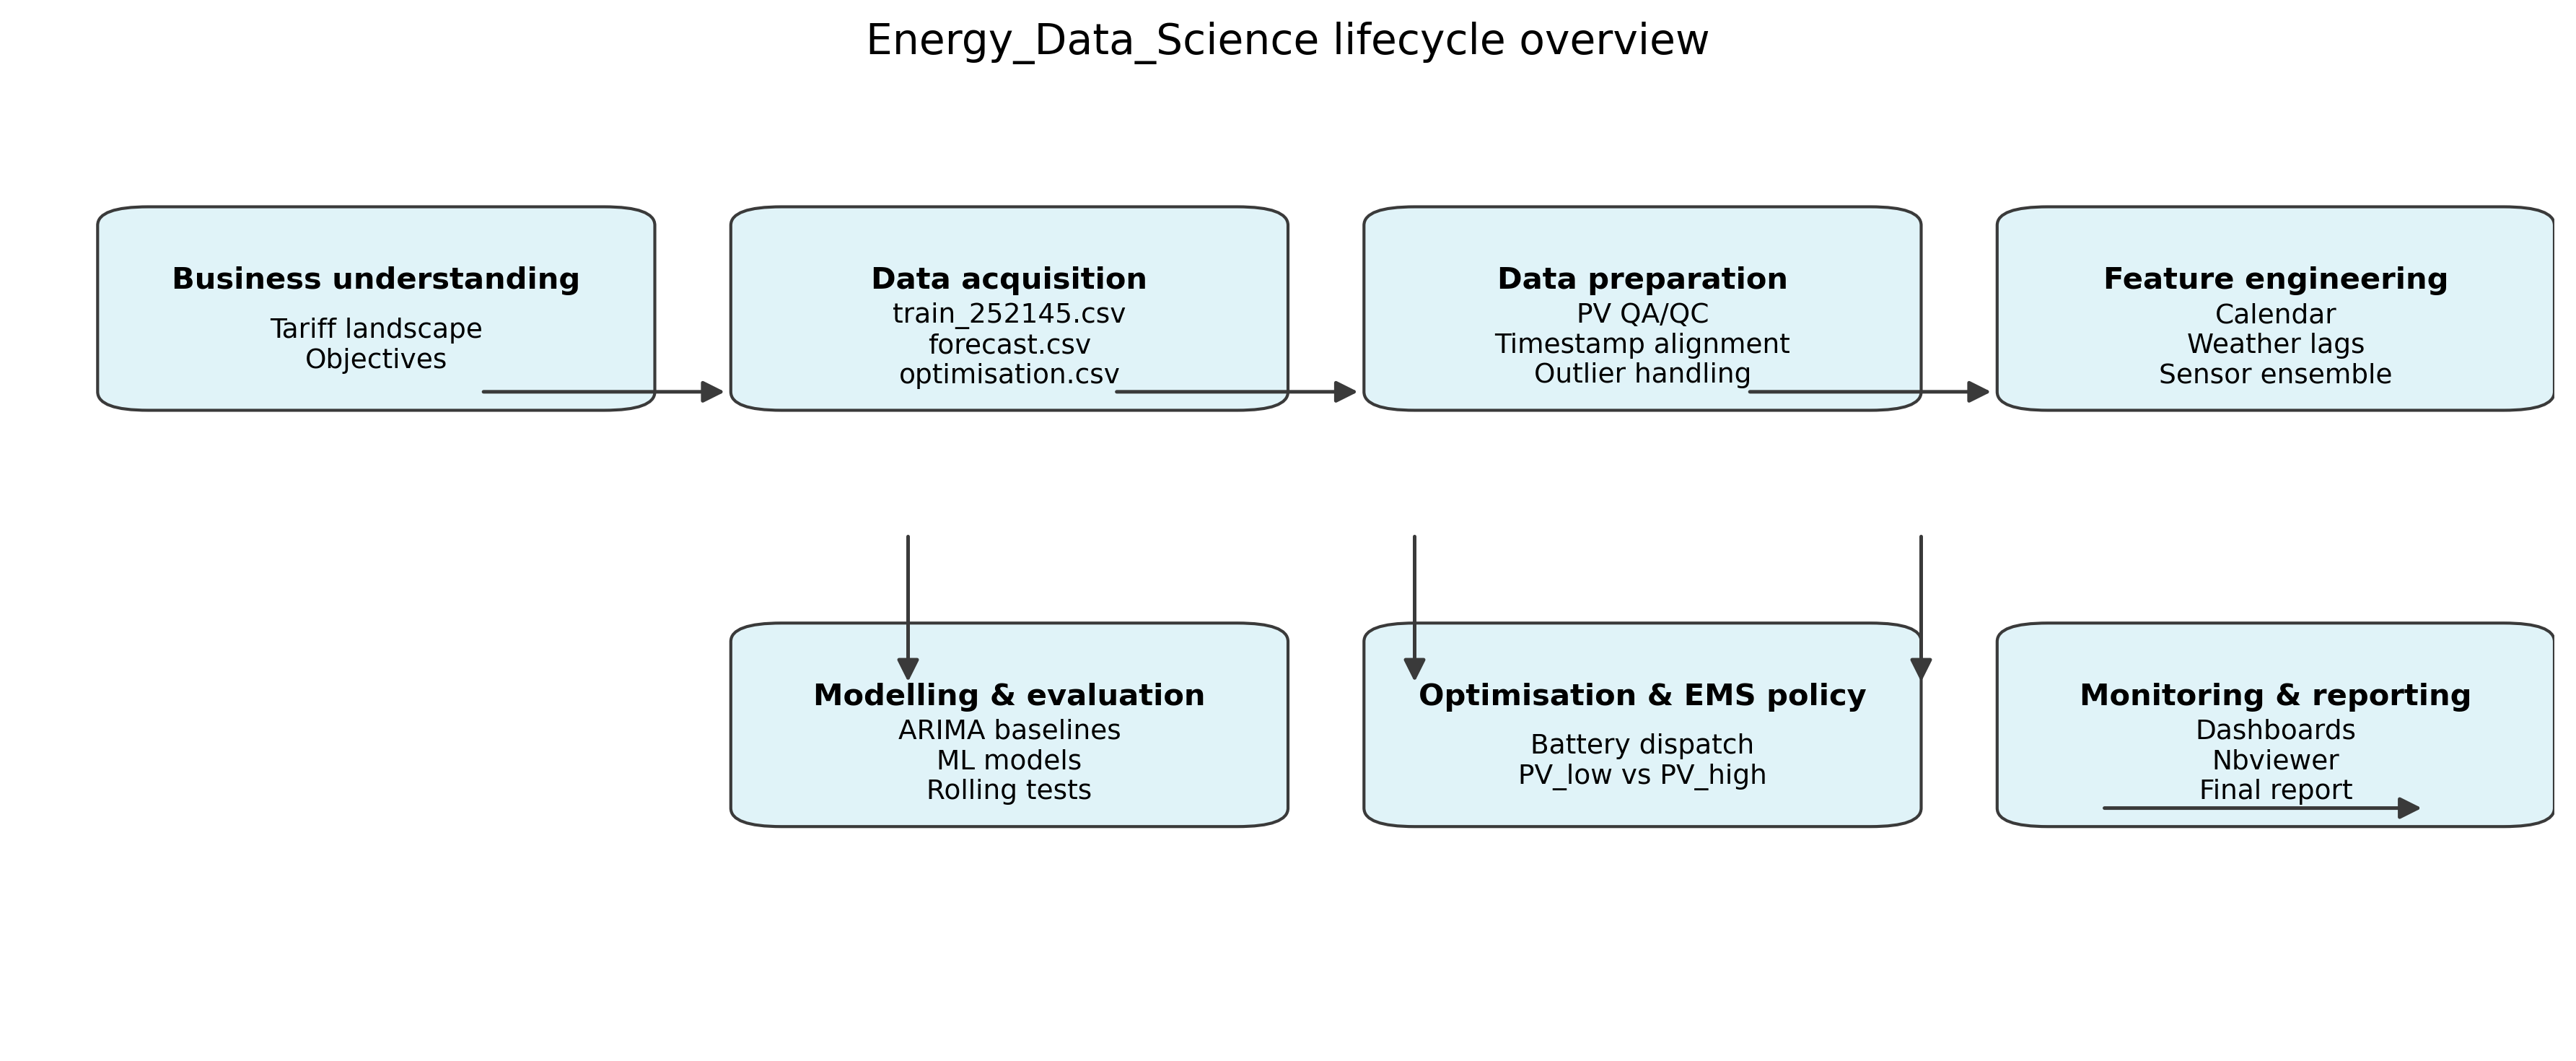
\includegraphics[width=\linewidth]{task2_lifecycle.png}
  \caption{Project plan and lifecycle.}
  \label{fig:lifecycle}
\end{figure}

%===========================
% 3. Data Exploration
%===========================
\section{Data Exploration and Visualization}
Exploratory analysis reveals strong diurnal seasonality and weekday effects. Distributional checks confirm PV skewness and demand spread; correlations indicate temperature and calendar relevance.

\begin{figure}[H]
  \centering
  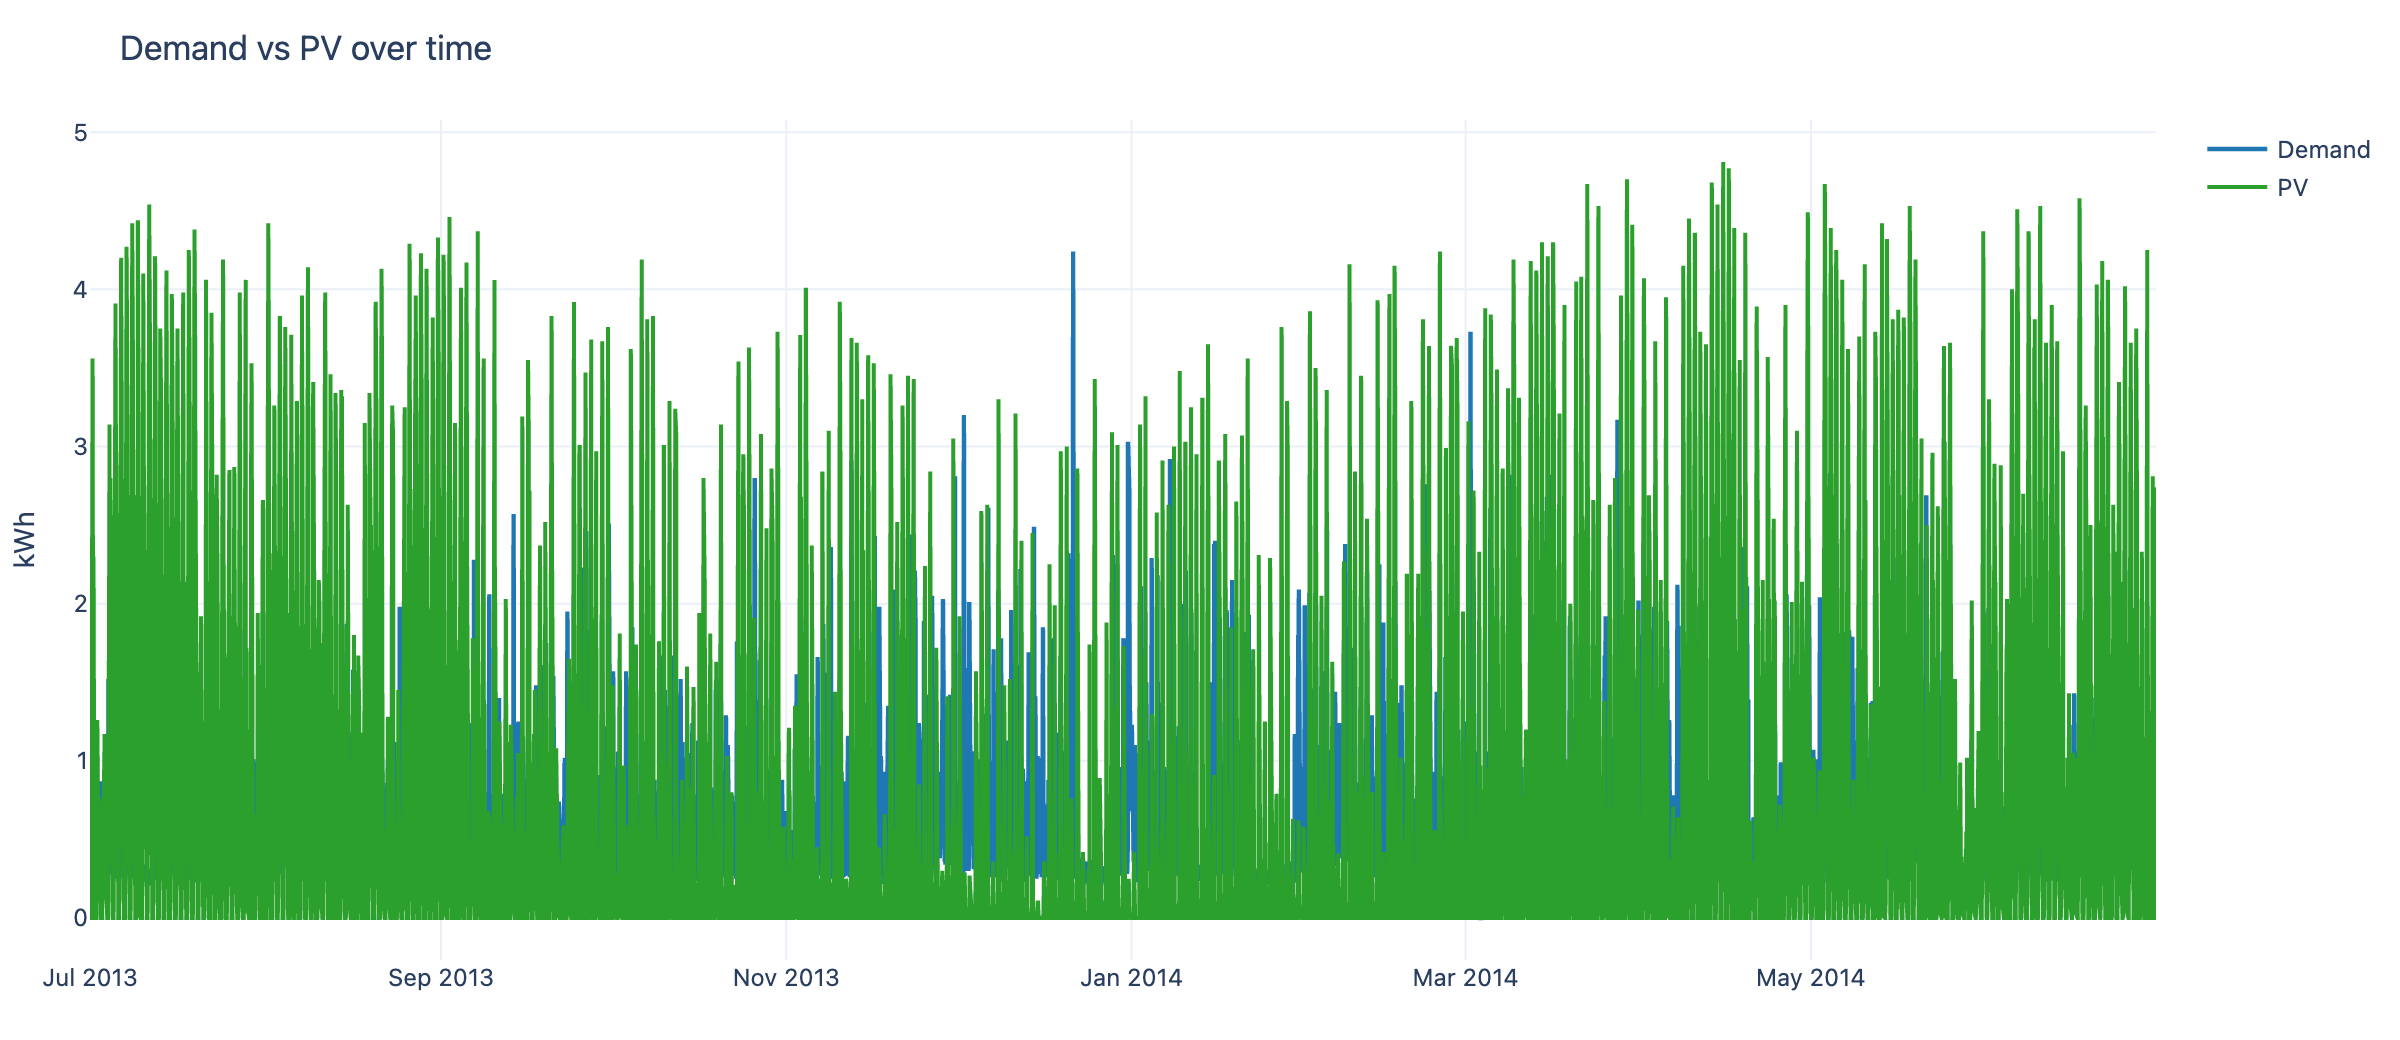
\includegraphics[width=\linewidth]{01_demand_pv_timeseries.png}
  \caption{Demand and PV overview time series.}
  \label{fig:timeseries_main}
\end{figure}

\begin{figure}[H]
  \centering
  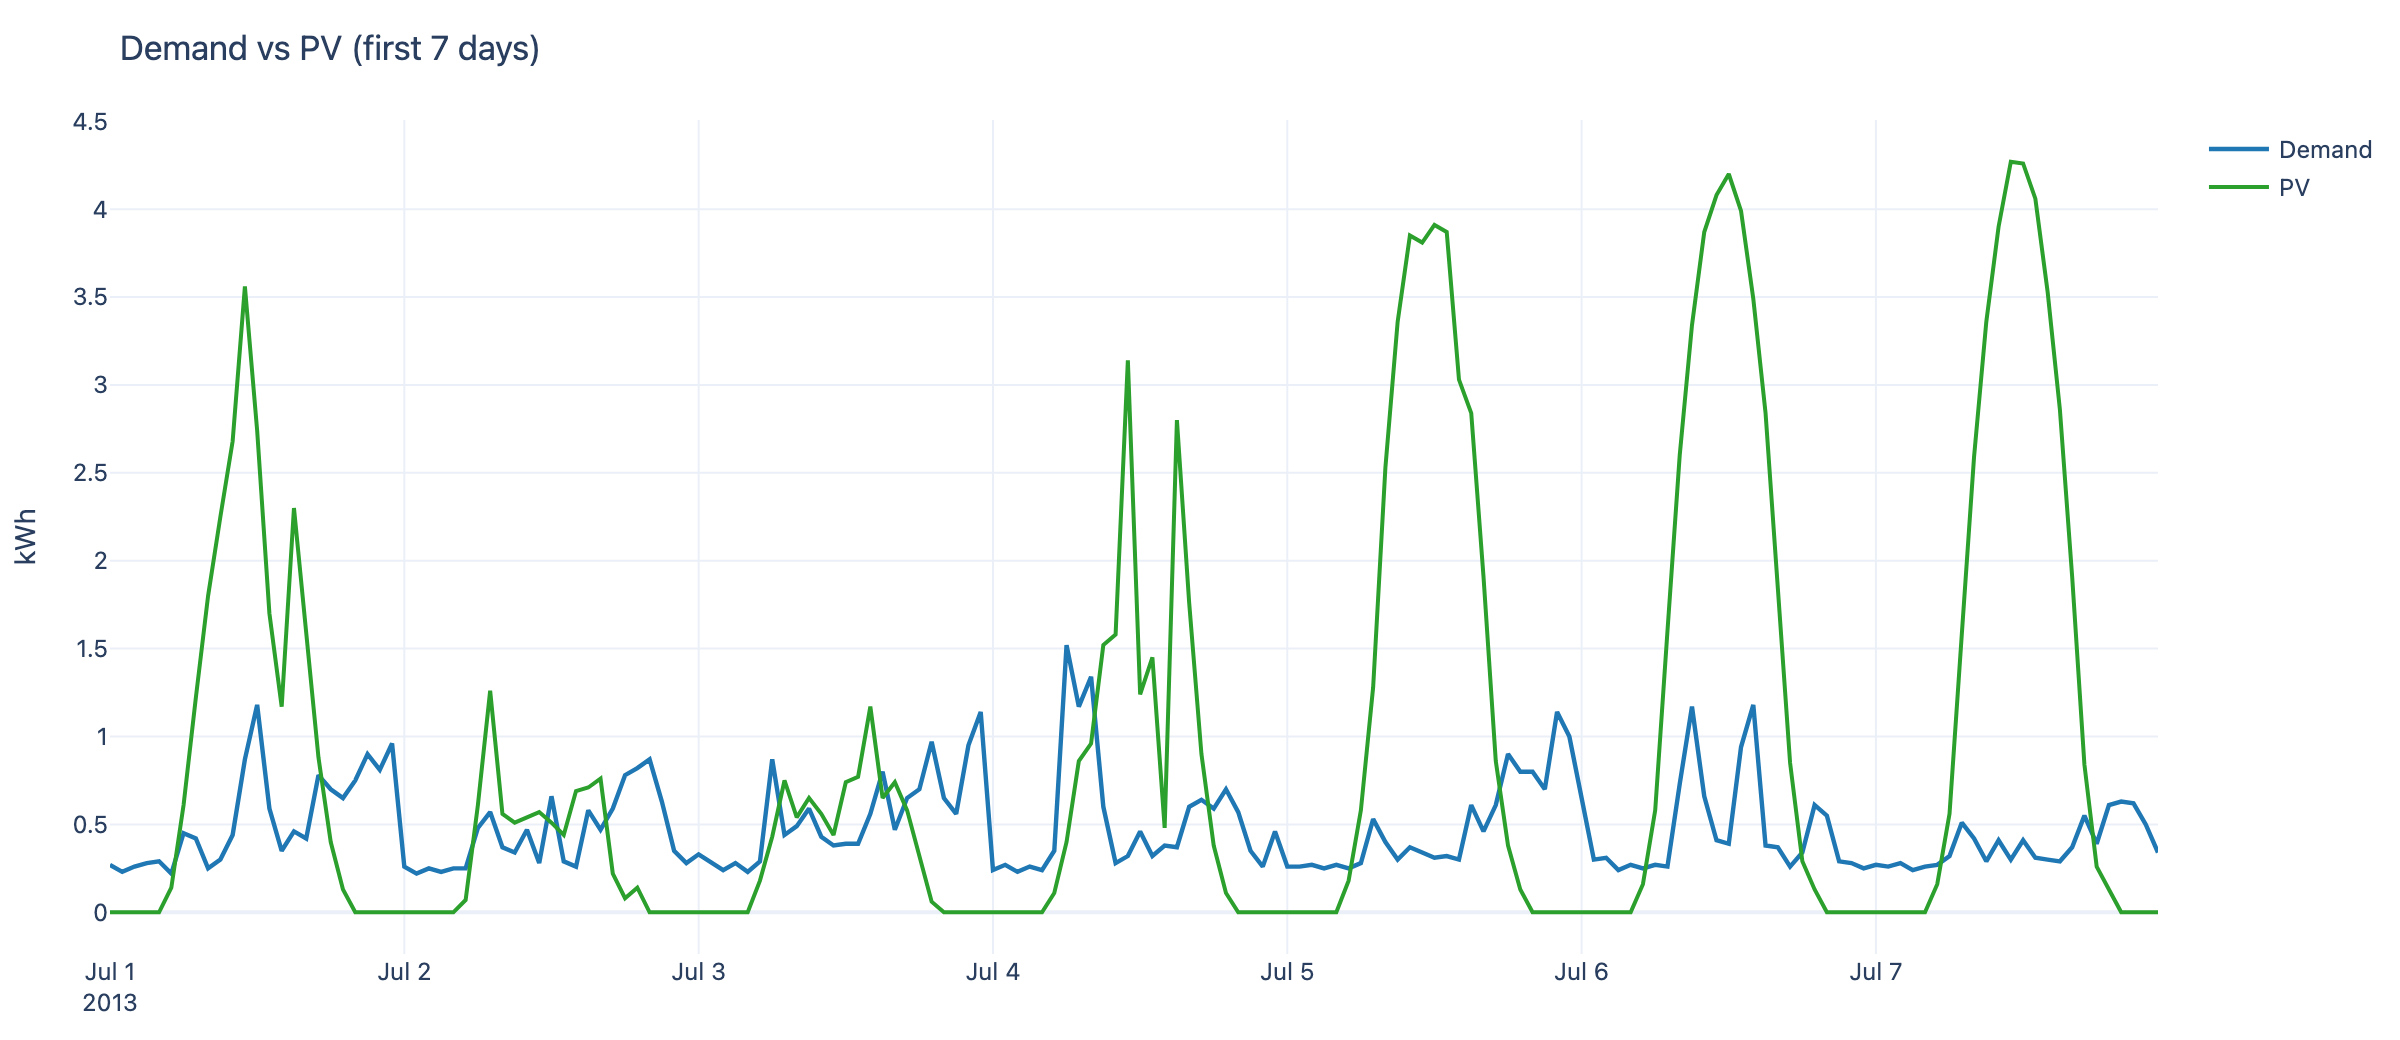
\includegraphics[width=\linewidth]{01_demand_pv_daily_sample.png}
  \caption{One-week demand and PV sample.}
  \label{fig:timeseries_week}
\end{figure}

\begin{figure}[H]
  \centering
  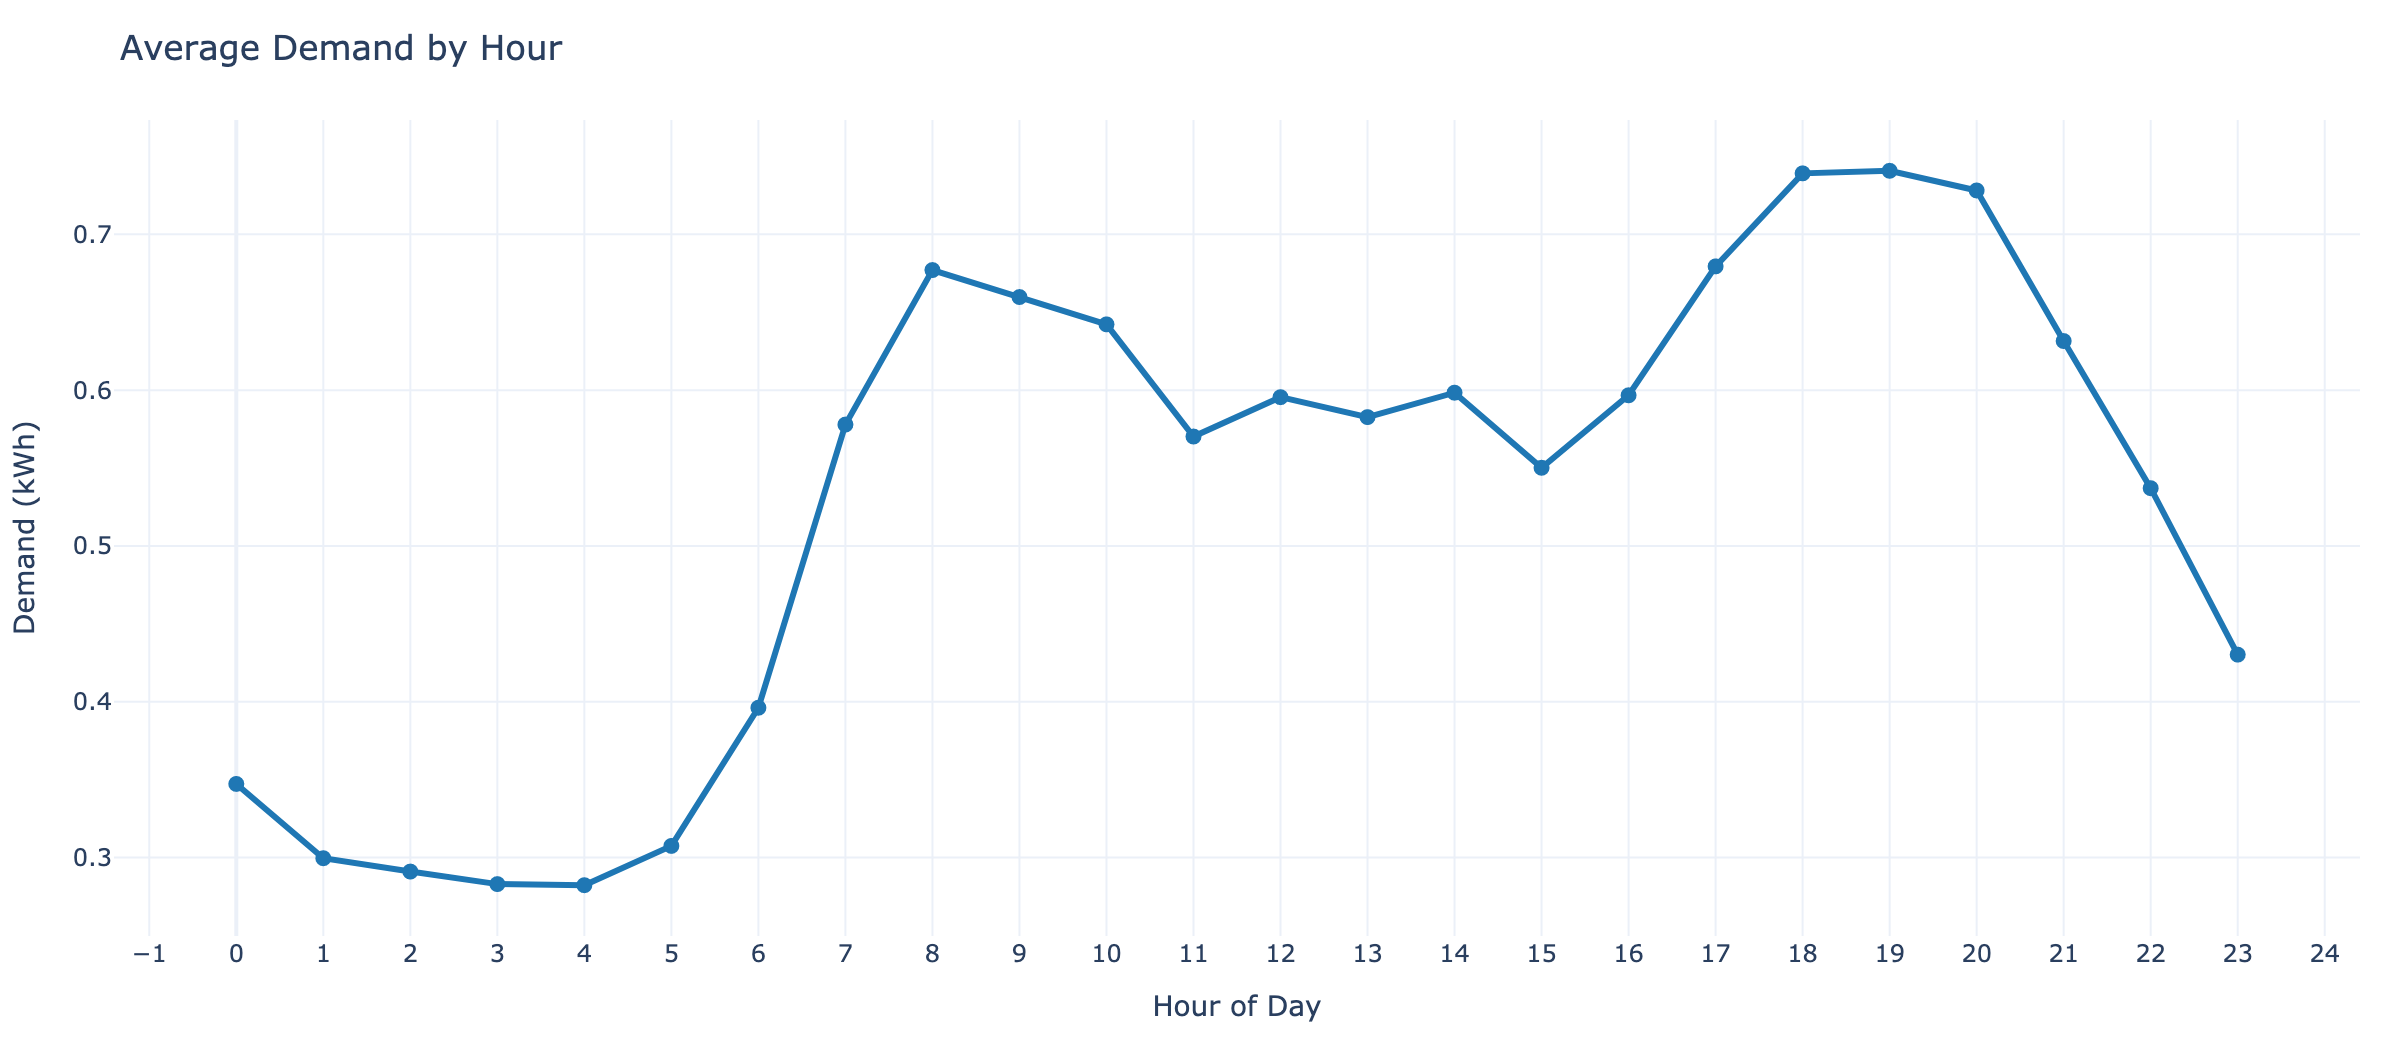
\includegraphics[width=\linewidth]{02_demand_diurnal_profile.png}
  \caption{Diurnal demand profile.}
  \label{fig:diurnal}
\end{figure}

\begin{figure}[H]
  \centering
  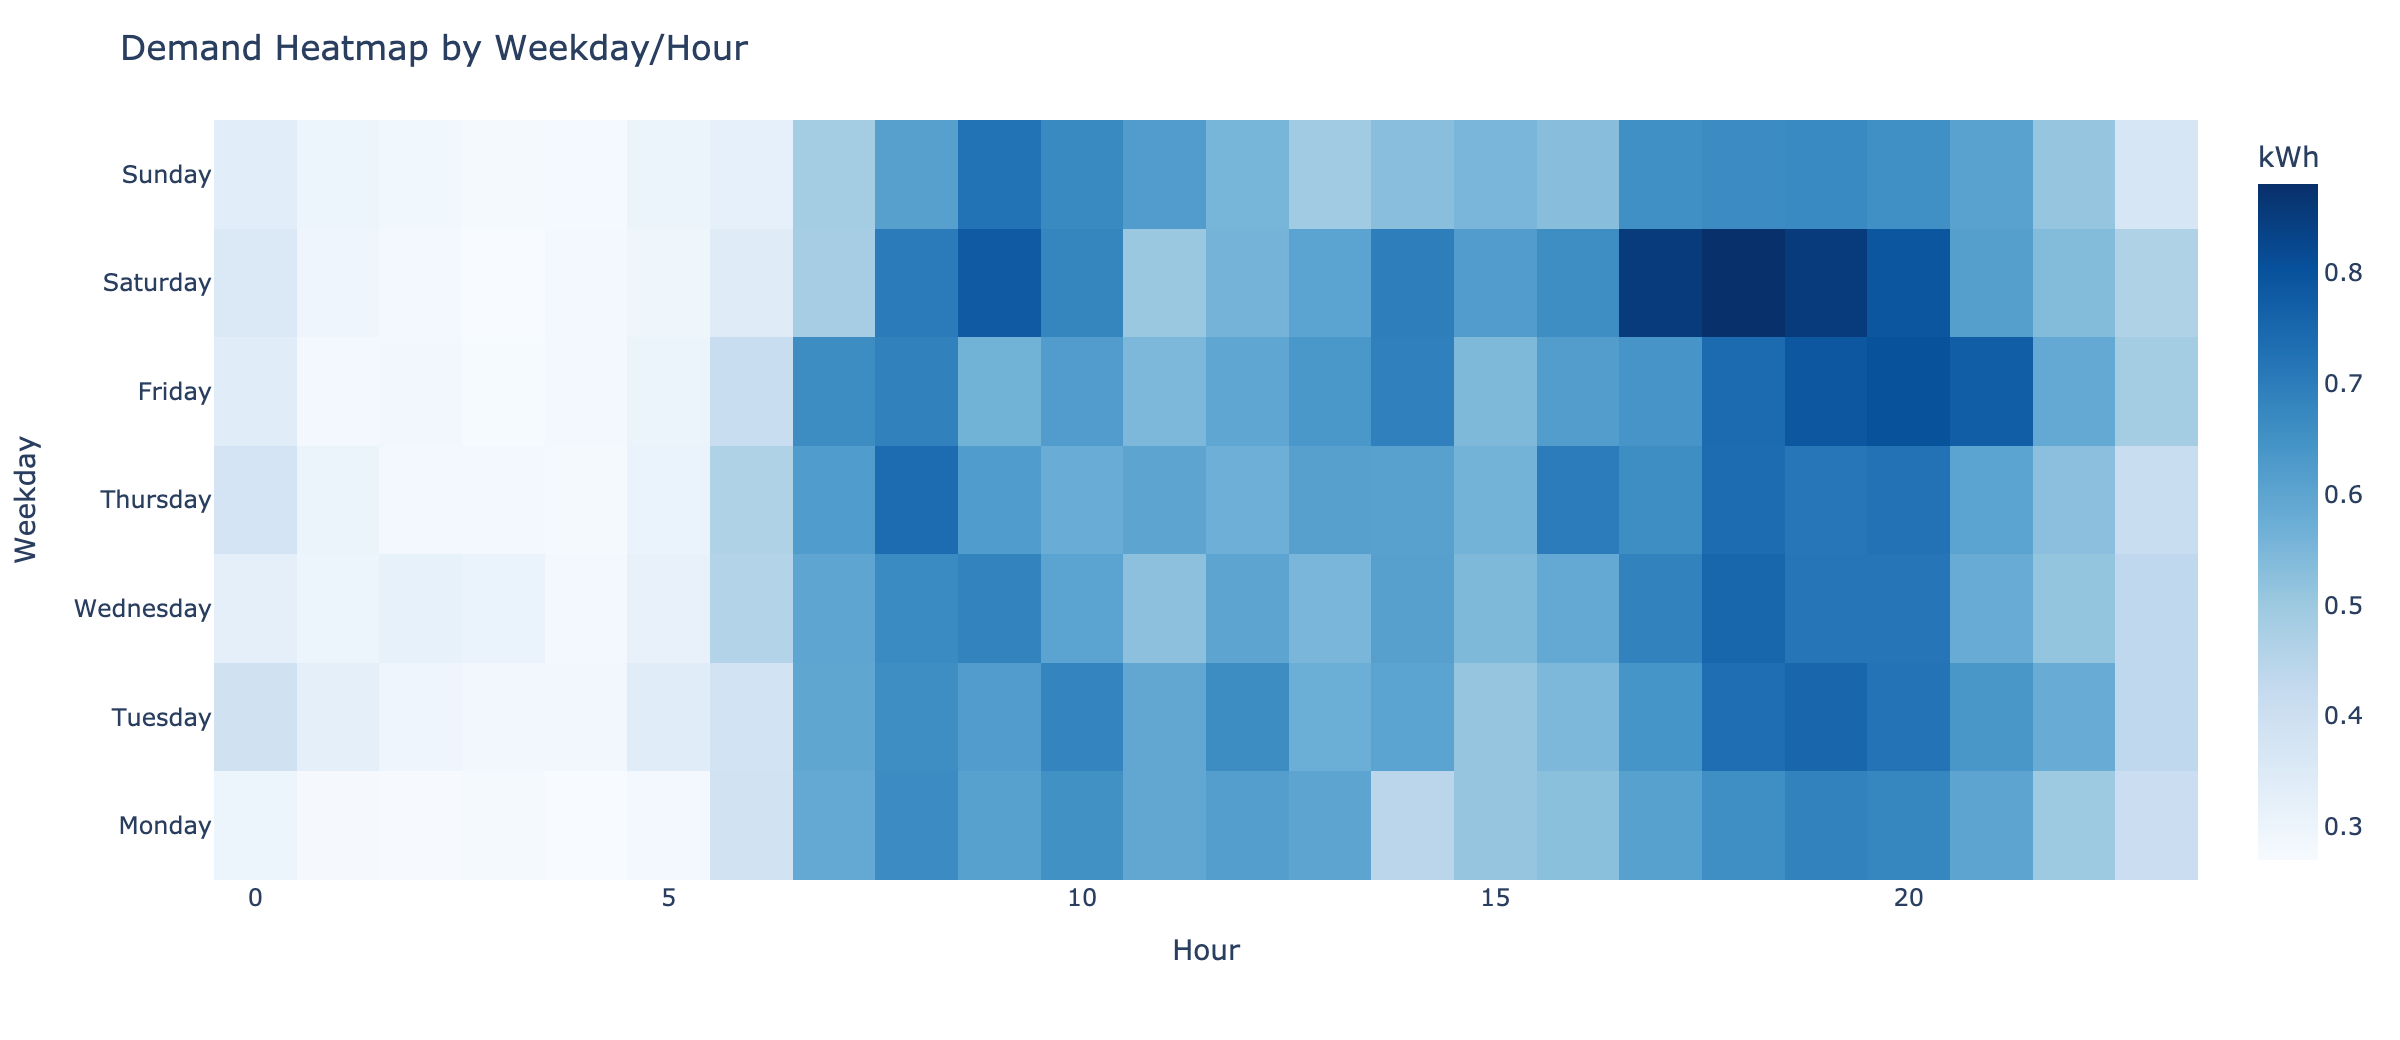
\includegraphics[width=\linewidth]{02_demand_weekday_heatmap.png}
  \caption{Weekday-hour heatmap of demand.}
  \label{fig:weekday_heatmap}
\end{figure}

%===========================
% 4. Cleaning
%===========================
\section{Data Cleaning and Preprocessing}
Cleaning tackled missingness, timestamp consistency, and PV corrections (bounding, smoothing). Missingness is visualized while PV quality metrics are summarized in tables.

\begin{figure}[H]
  \centering
  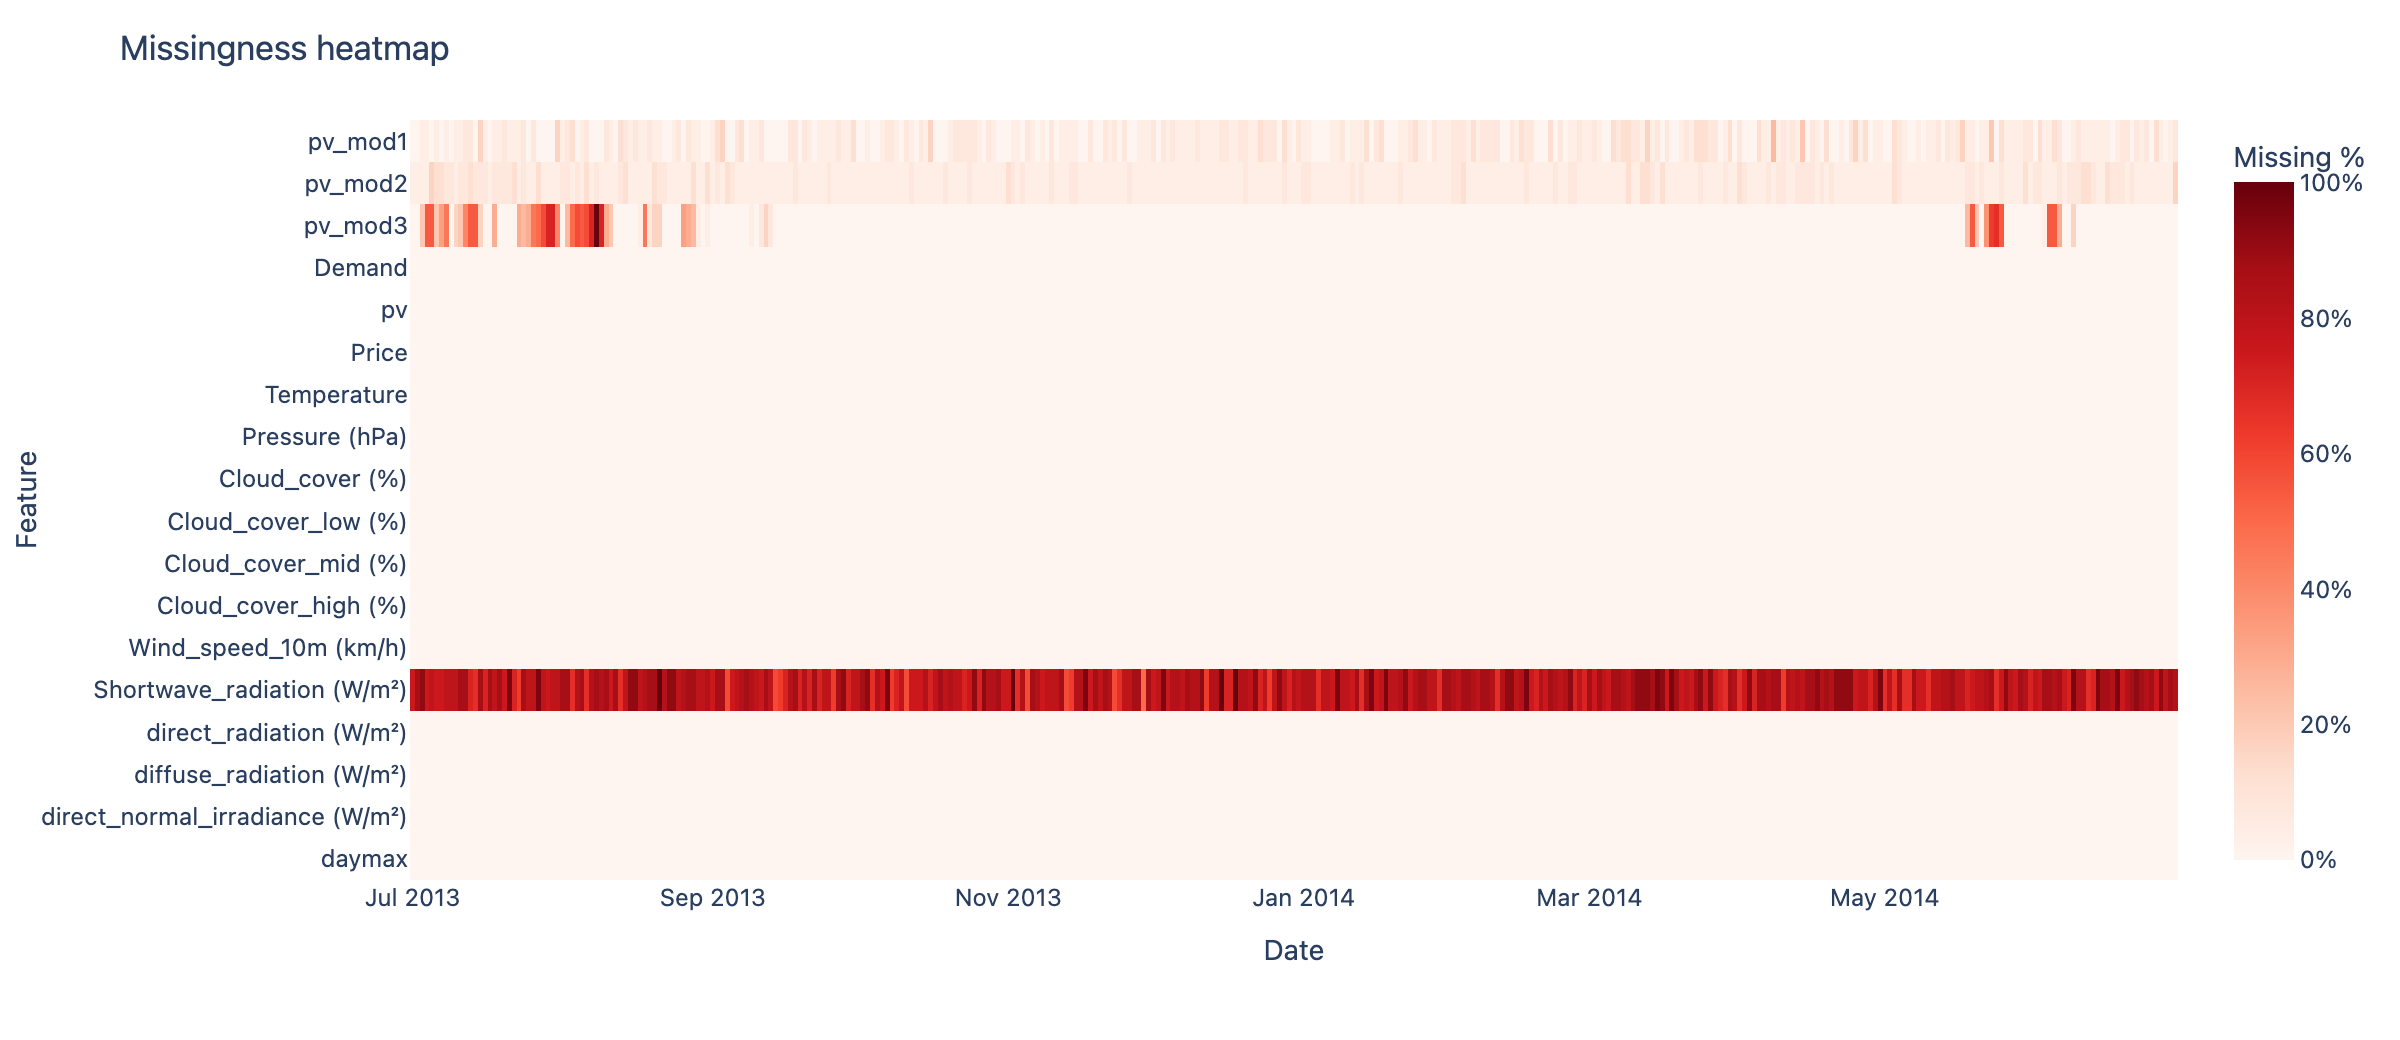
\includegraphics[width=\linewidth]{04_missingness_heatmap.png}
  \caption{Missingness heatmap by feature and time.}
  \label{fig:missingness}
\end{figure}

\begin{table}[H]
  \centering
  \caption{PV gap statistics (share of missing and zero values).}
  \label{tab:pv_gap}
  \begin{tabular}{lrrrr}
  \toprule
  Column & Missing (\%) & Zero (\%) & Mean & Std \\
  \midrule
  \multicolumn{5}{c}{See reports/tables/04\_pv\_gap\_stats.csv for full table} \\
  \bottomrule
  \end{tabular}
\end{table}

%===========================
% 5. Feature Engineering
%===========================
\section{Feature Engineering}
Calendar, lagged, and rolling-window features were engineered. Feature distributions were checked; proxy importance shown below.

\begin{figure}[H]
  \centering
  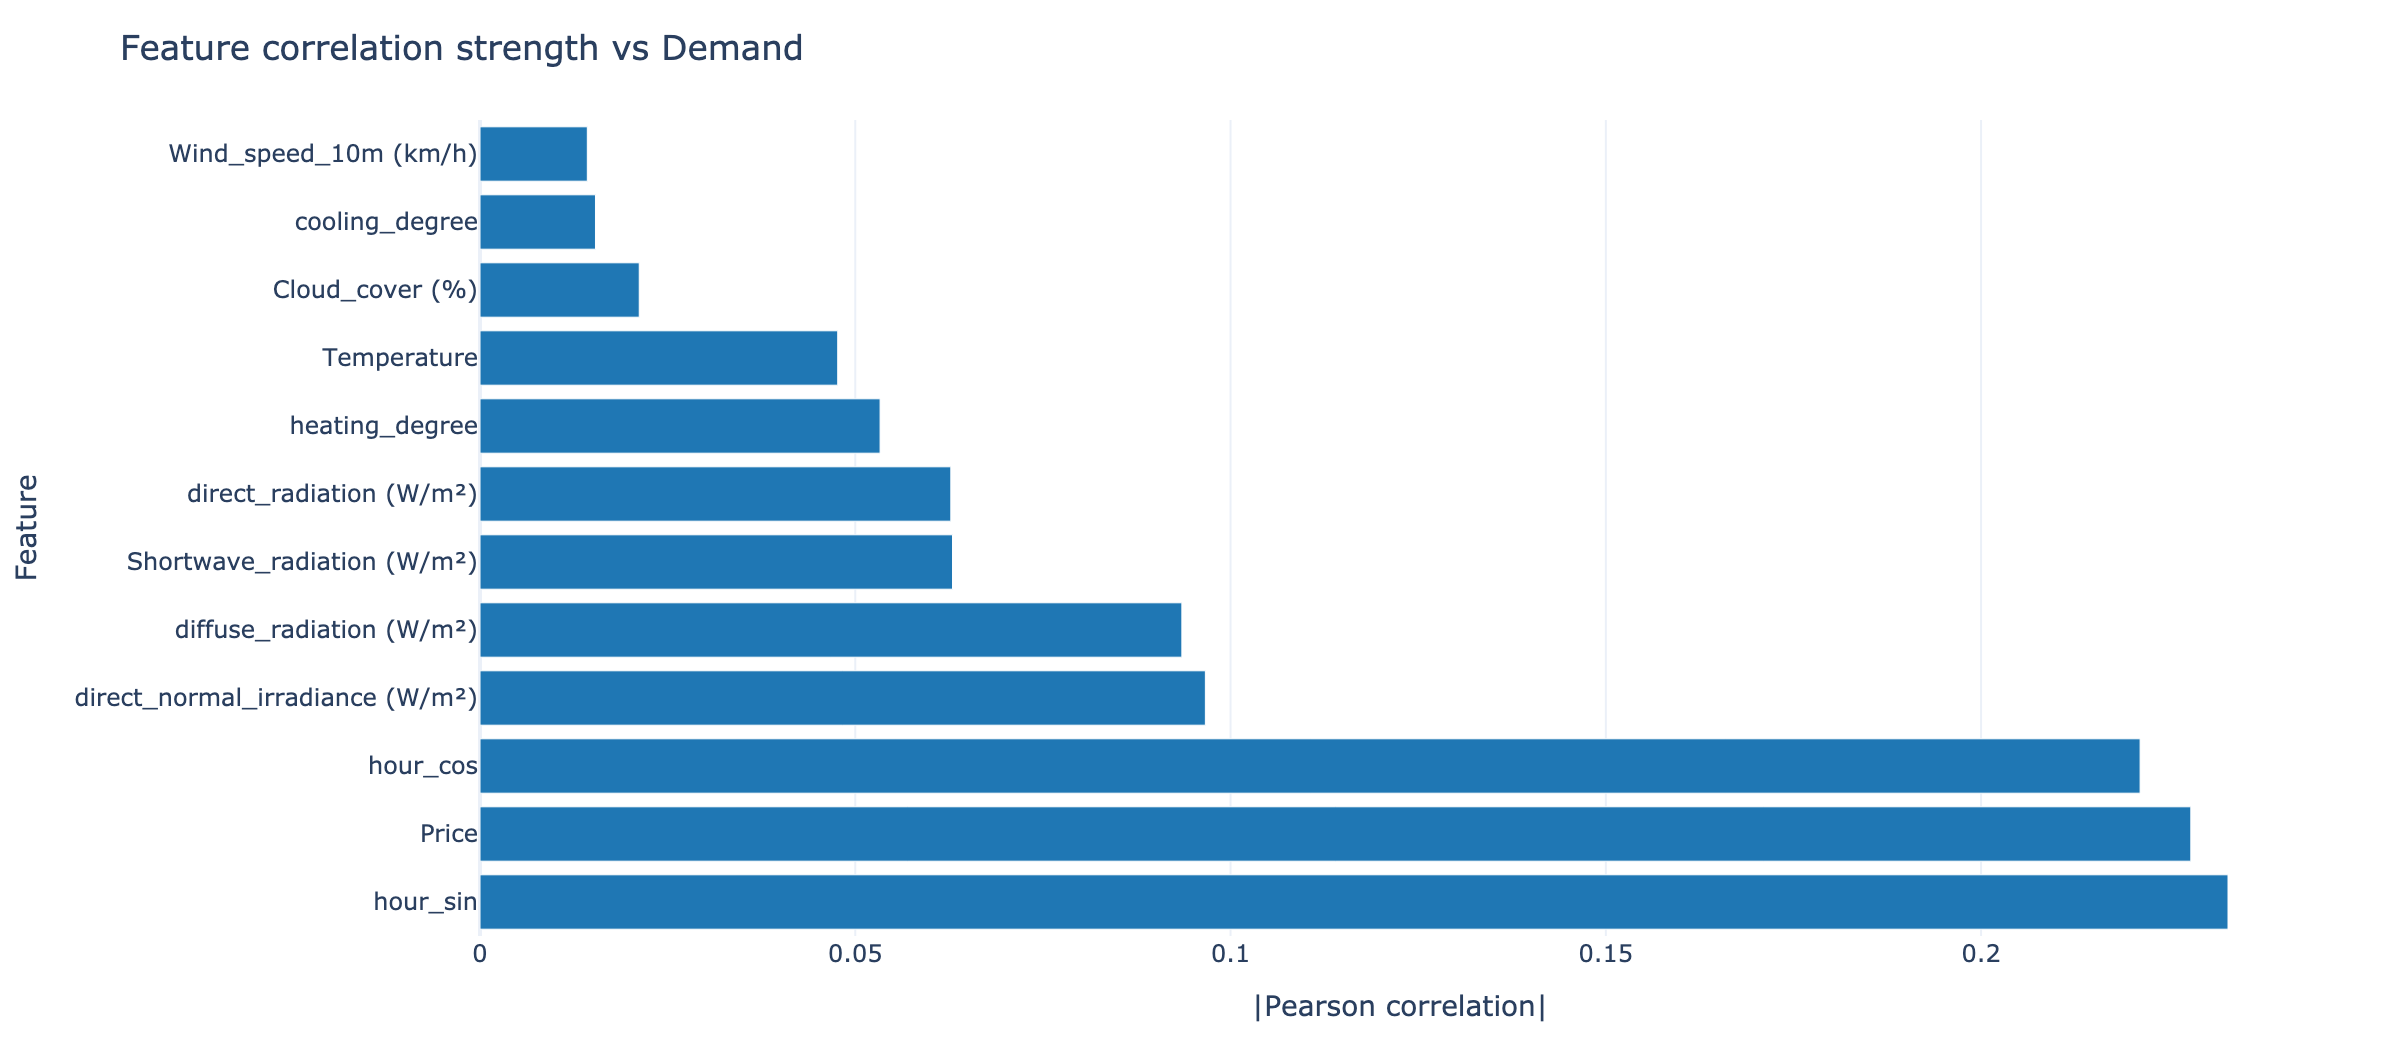
\includegraphics[width=\linewidth]{05_feature_importance.png}
  \caption{Feature importance proxy (correlation strength to Demand).}
  \label{fig:feat_importance}
\end{figure}

%===========================
% 6. Time Series Analysis
%===========================
\section{Time Series Analysis}
We applied STL decomposition to Demand: $y_t = T_t + S_t + R_t$. Diurnal seasonality is dominant with moderate weekly effects.

\begin{figure}[H]
  \centering
  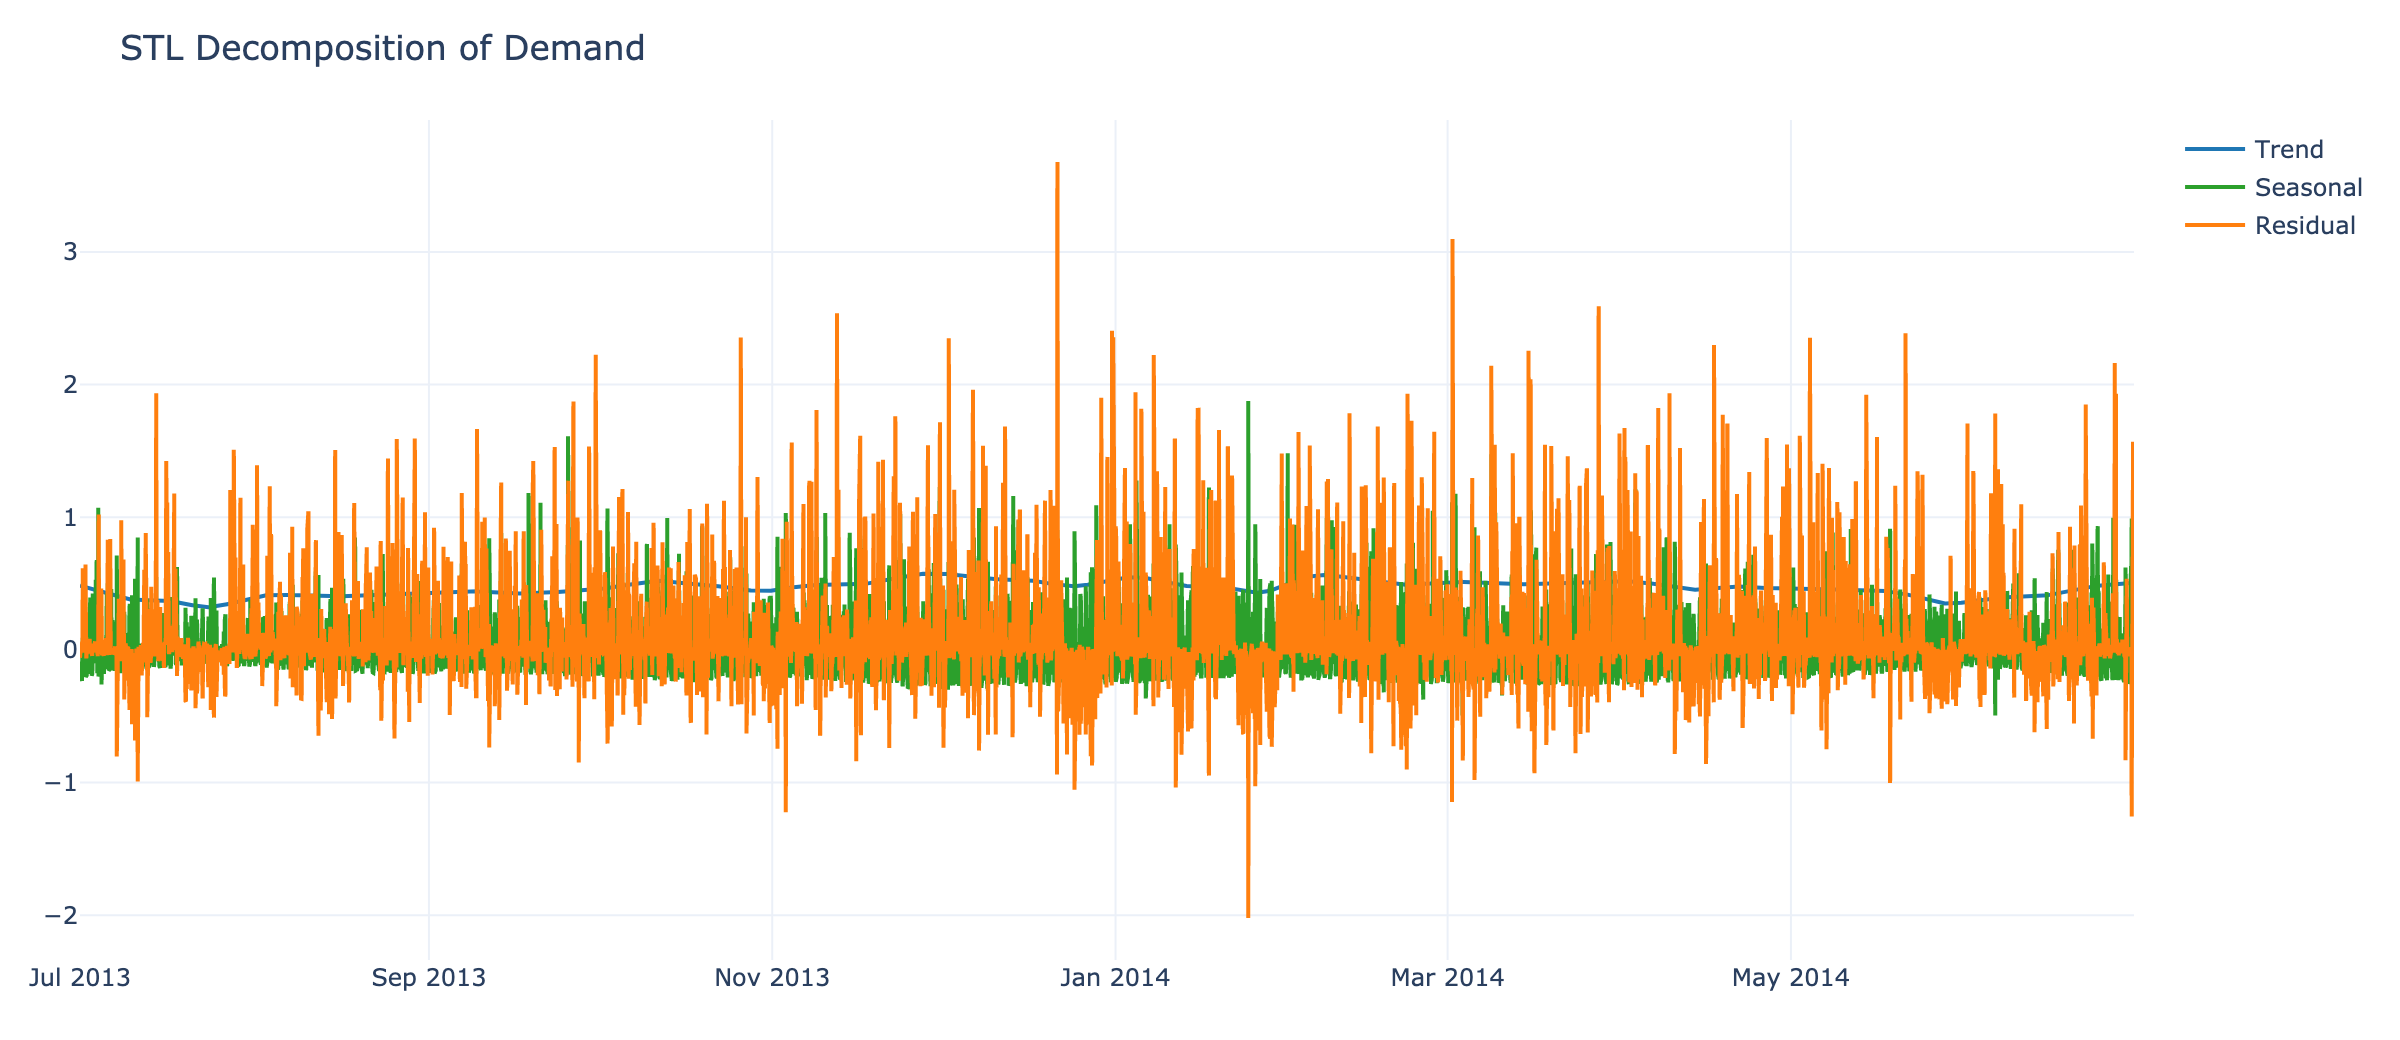
\includegraphics[width=\linewidth]{03_demand_seasonality_stl.png}
  \caption{Demand seasonality decomposition using STL.}
  \label{fig:stl}
\end{figure}

%===========================
% 7. Statistical Modelling
%===========================
\section{Statistical Modelling}
ACF/PACF diagnostics informed ARMA/ARIMA orders. A general ARIMA($p,d,q$) is $\Phi_p(B) (1 - B)^d y_t = \Theta_q(B) \varepsilon_t$.

\begin{figure}[H]
  \centering
  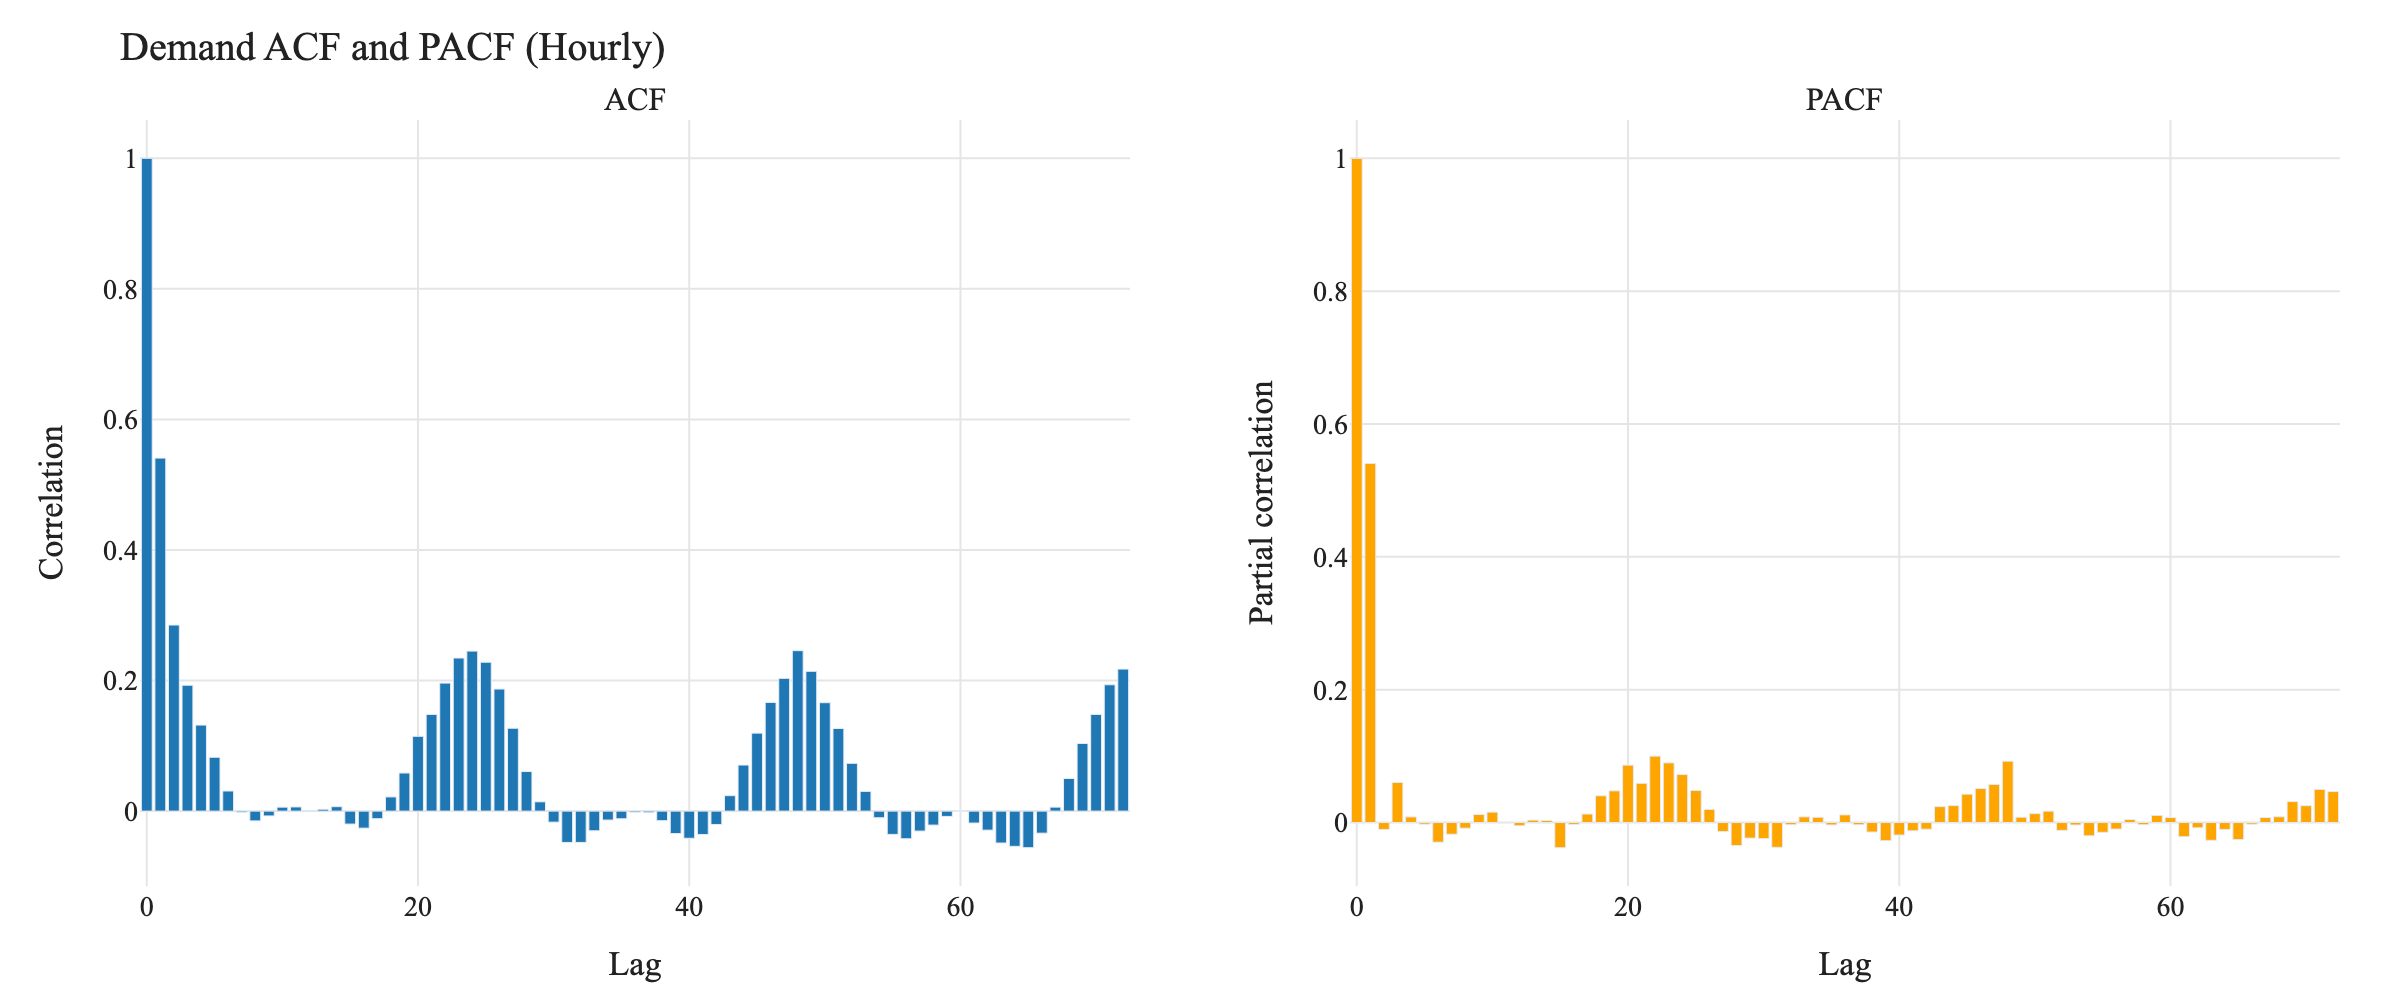
\includegraphics[width=\linewidth]{stats_acf_pacf.png}
  \caption{ACF/PACF diagnostics for model selection.}
  \label{fig:acf_pacf}
\end{figure}

\begin{figure}[H]
  \centering
  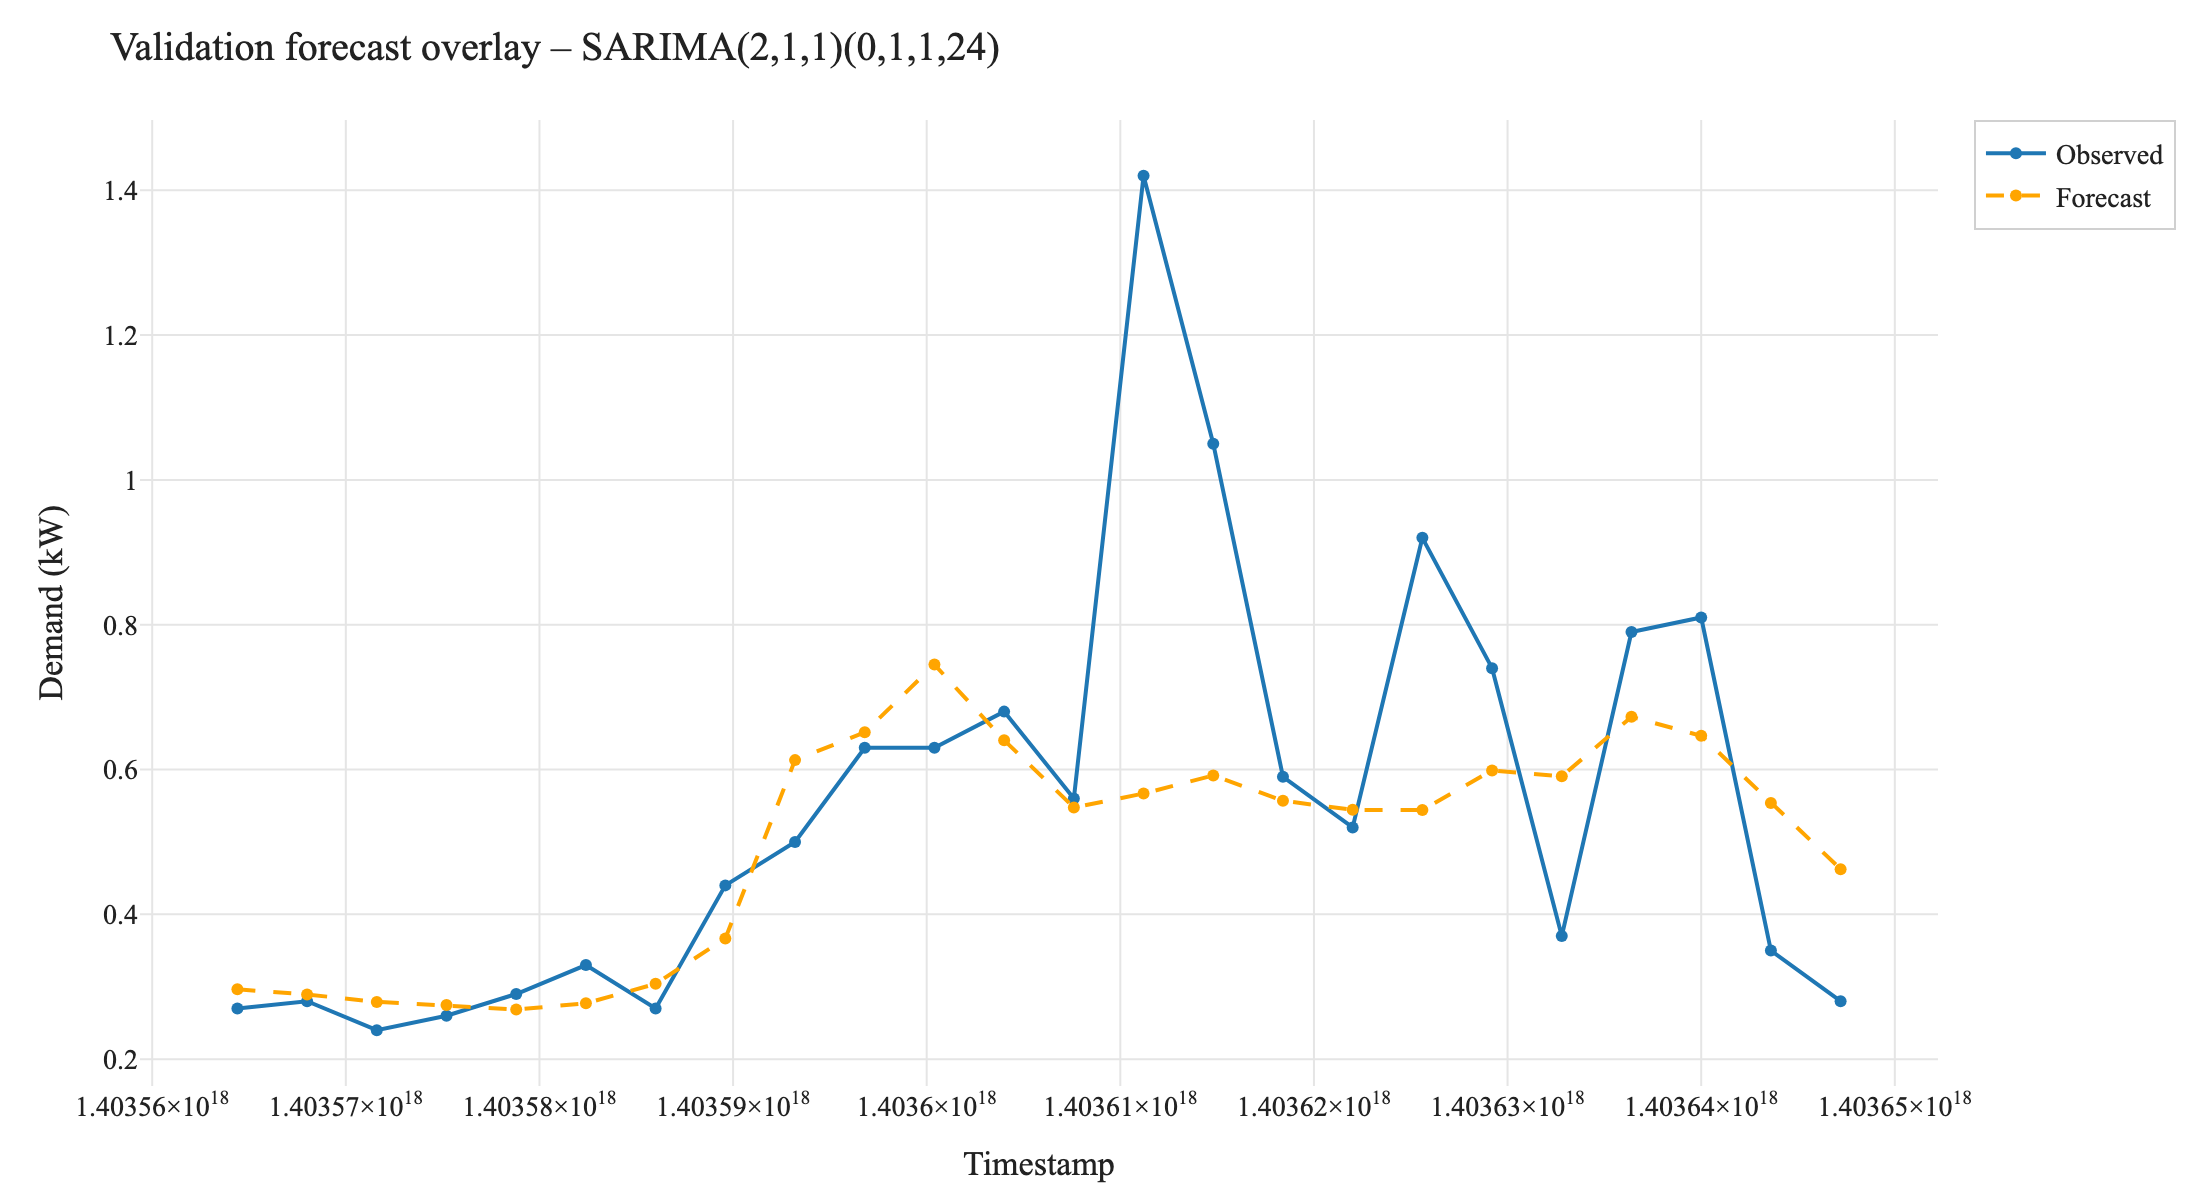
\includegraphics[width=\linewidth]{stats_forecast_overlay_best.png}
  \caption{Forecast overlay for best statistical model.}
  \label{fig:stats_best}
\end{figure}

\begin{figure}[H]
  \centering
  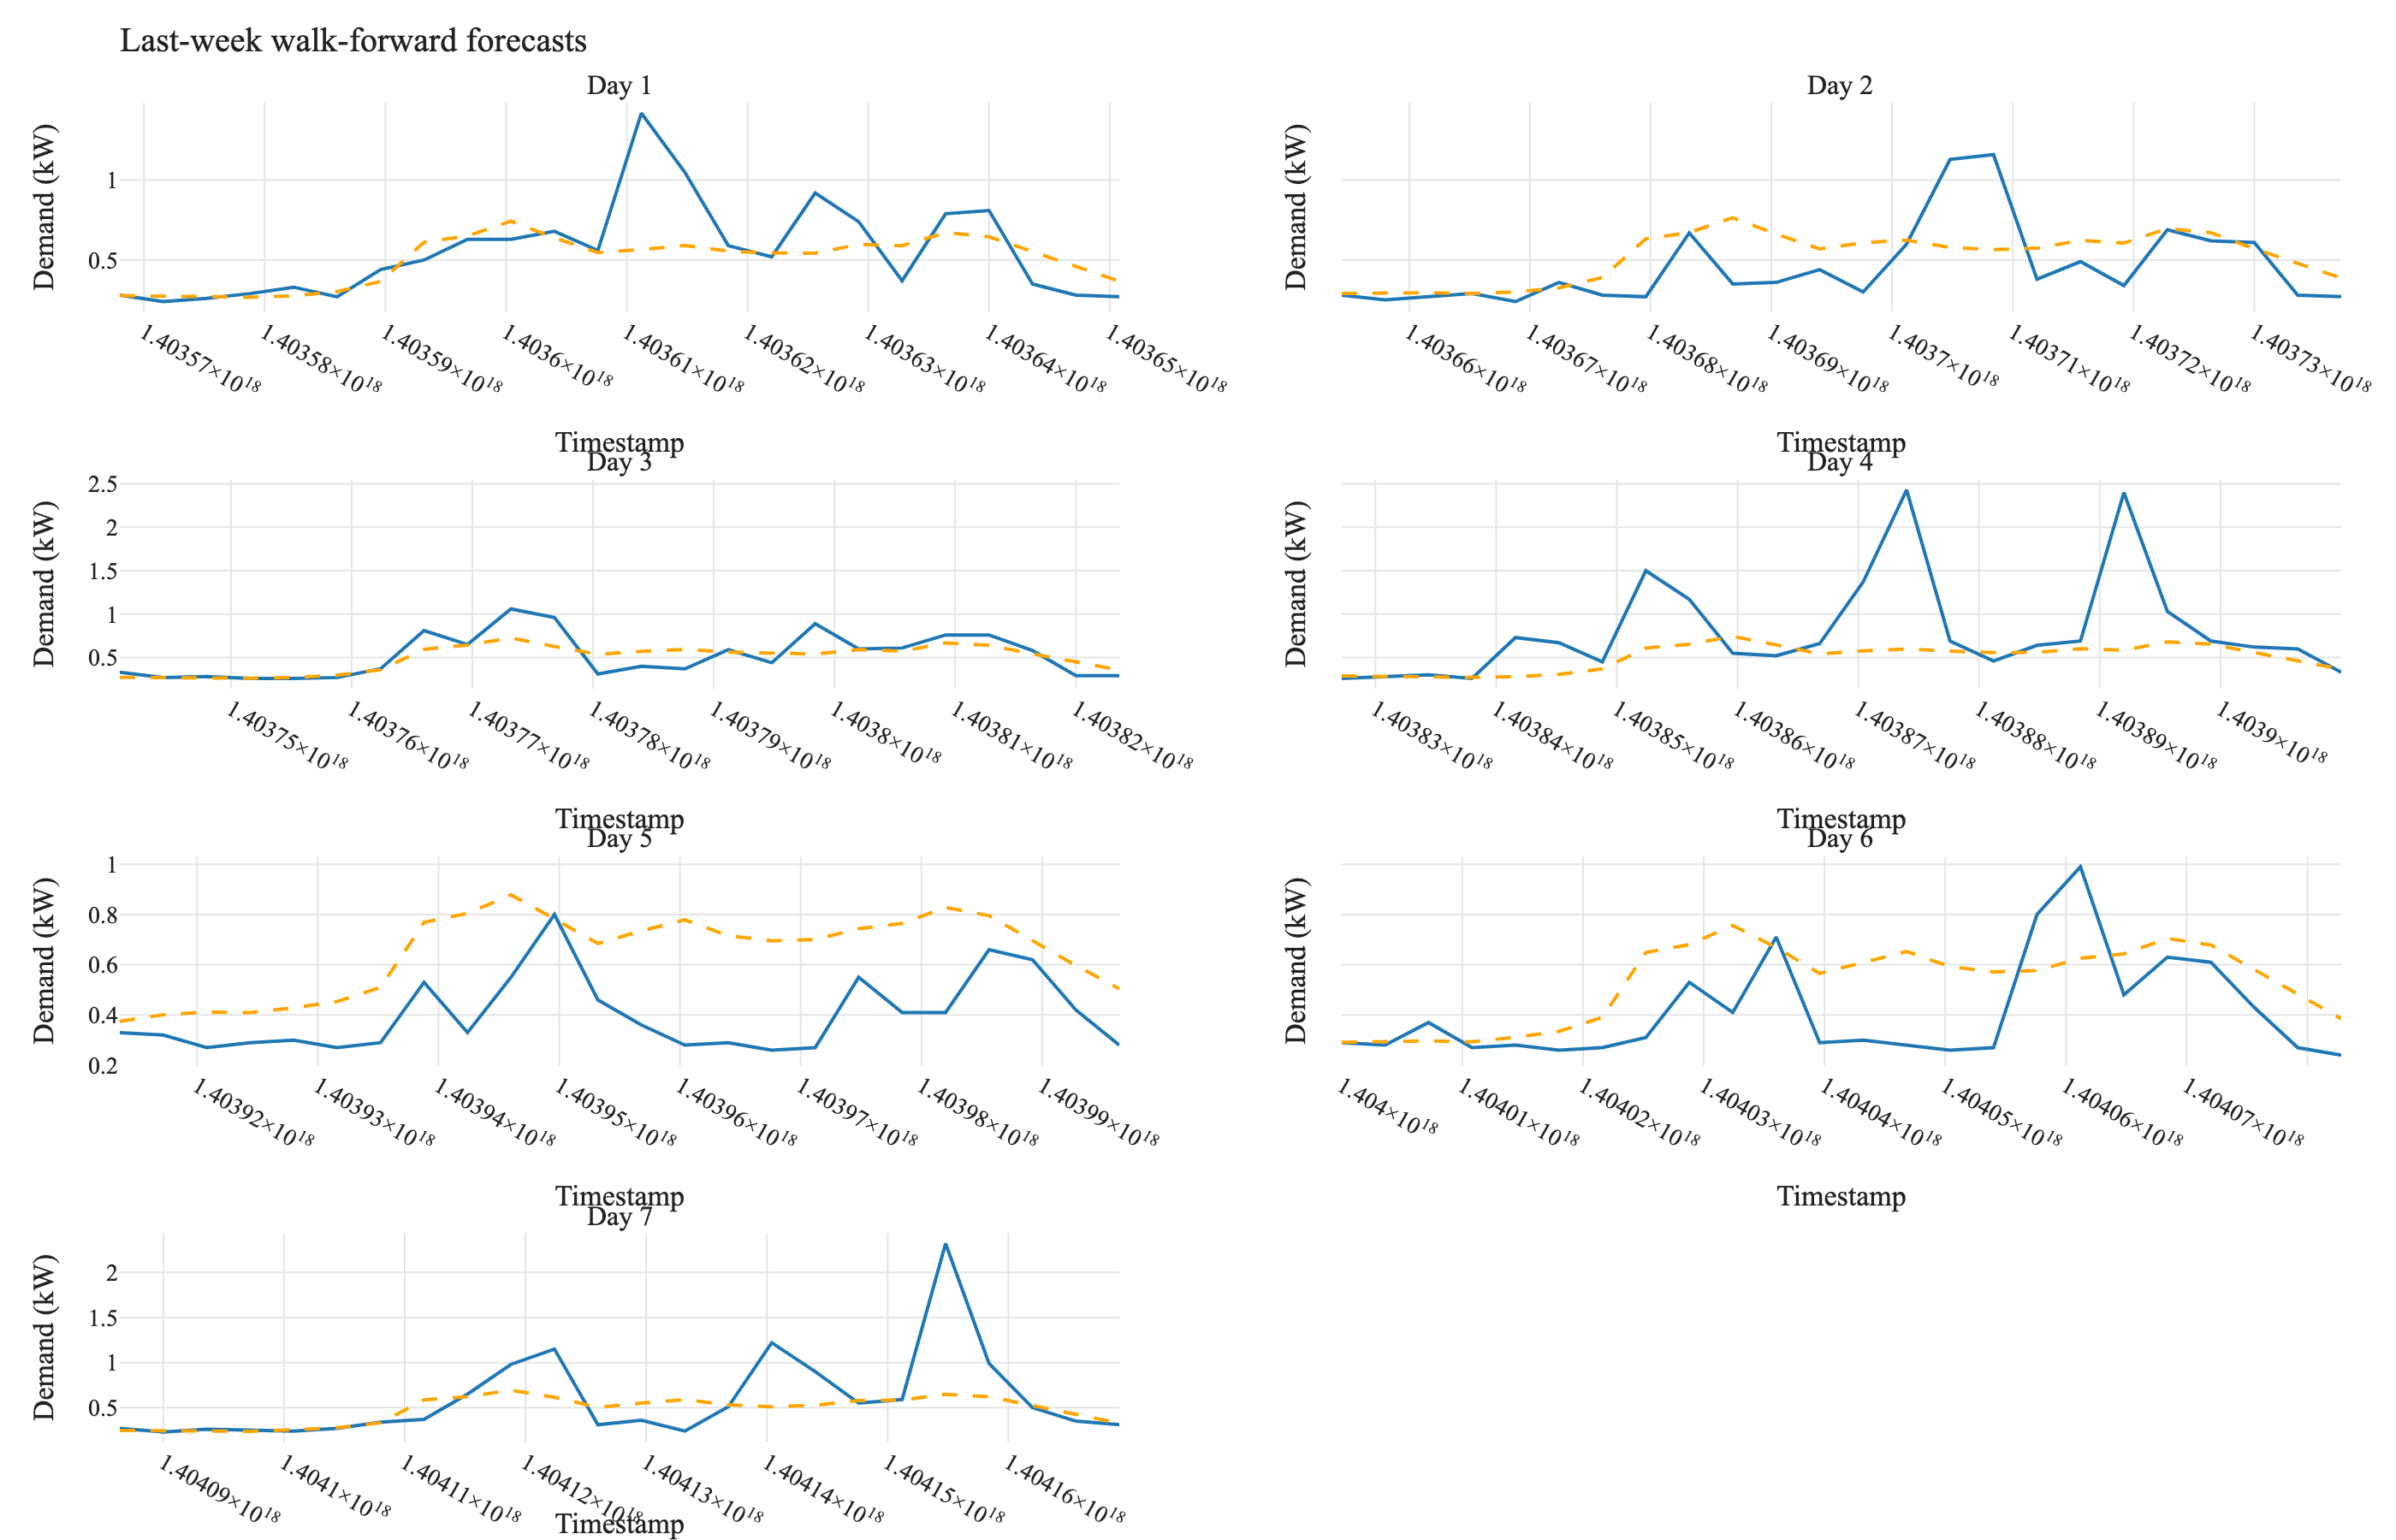
\includegraphics[width=\linewidth]{stats_walkforward_panels.png}
  \caption{Walk-forward evaluation panels for statistical models.}
  \label{fig:walkforward}
\end{figure}

\begin{figure}[H]
  \centering
  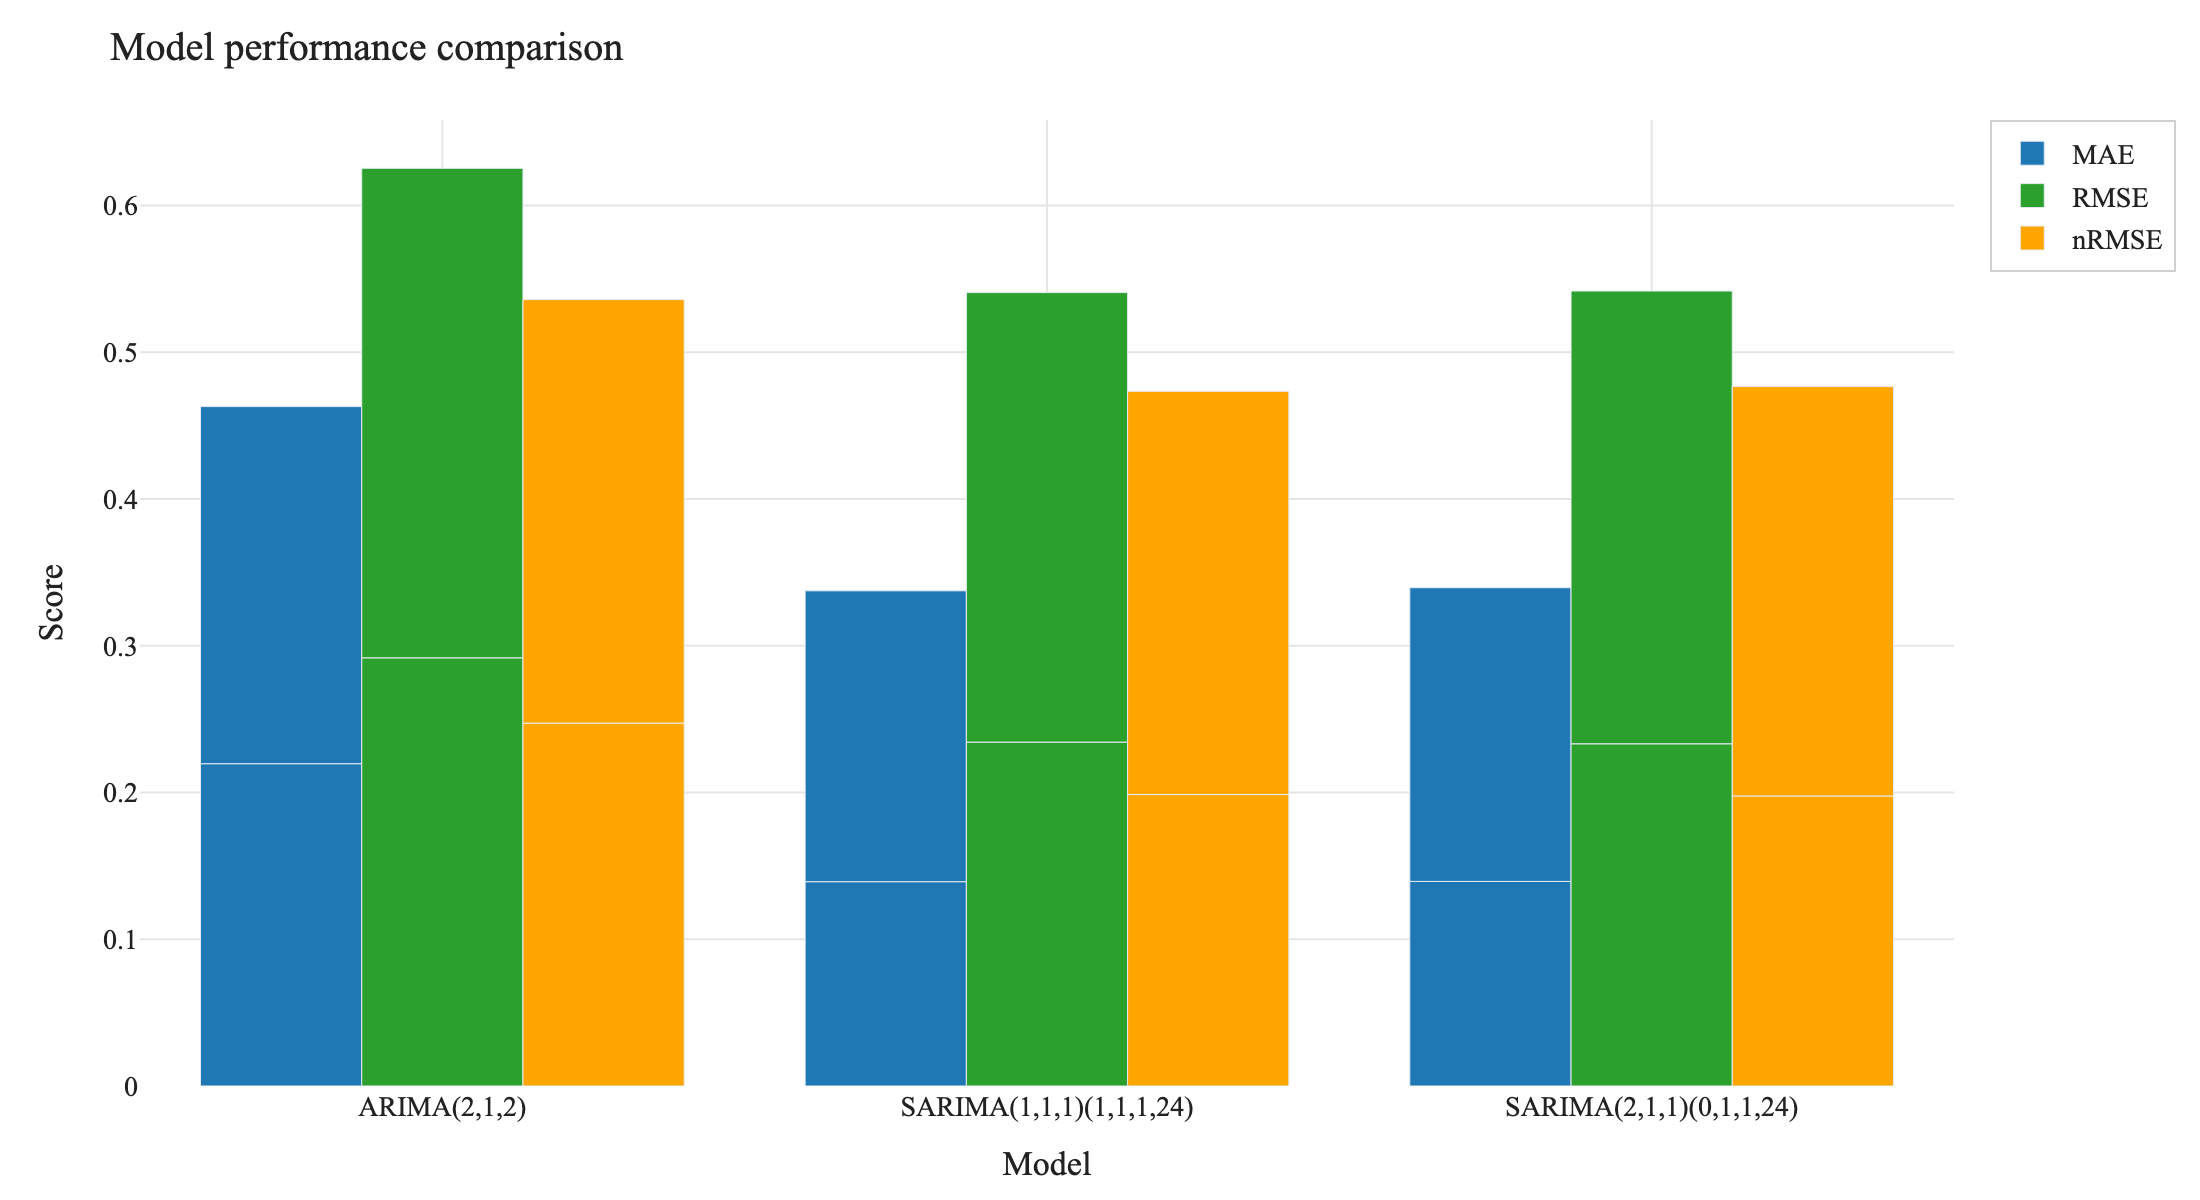
\includegraphics[width=\linewidth]{stats_metrics_bar.png}
  \caption{Metrics comparison (RMSE/MAE) across candidates.}
  \label{fig:stats_metrics}
\end{figure}

%===========================
% 8. Machine Learning
%===========================
\section{Machine Learning Modelling}
Supervised learners (e.g., gradient boosting, random forests) trained on engineered features. Cross-validation tuned hyperparameters; learning curves and importance plots indicate stable generalization.

\begin{figure}[H]
  \centering
  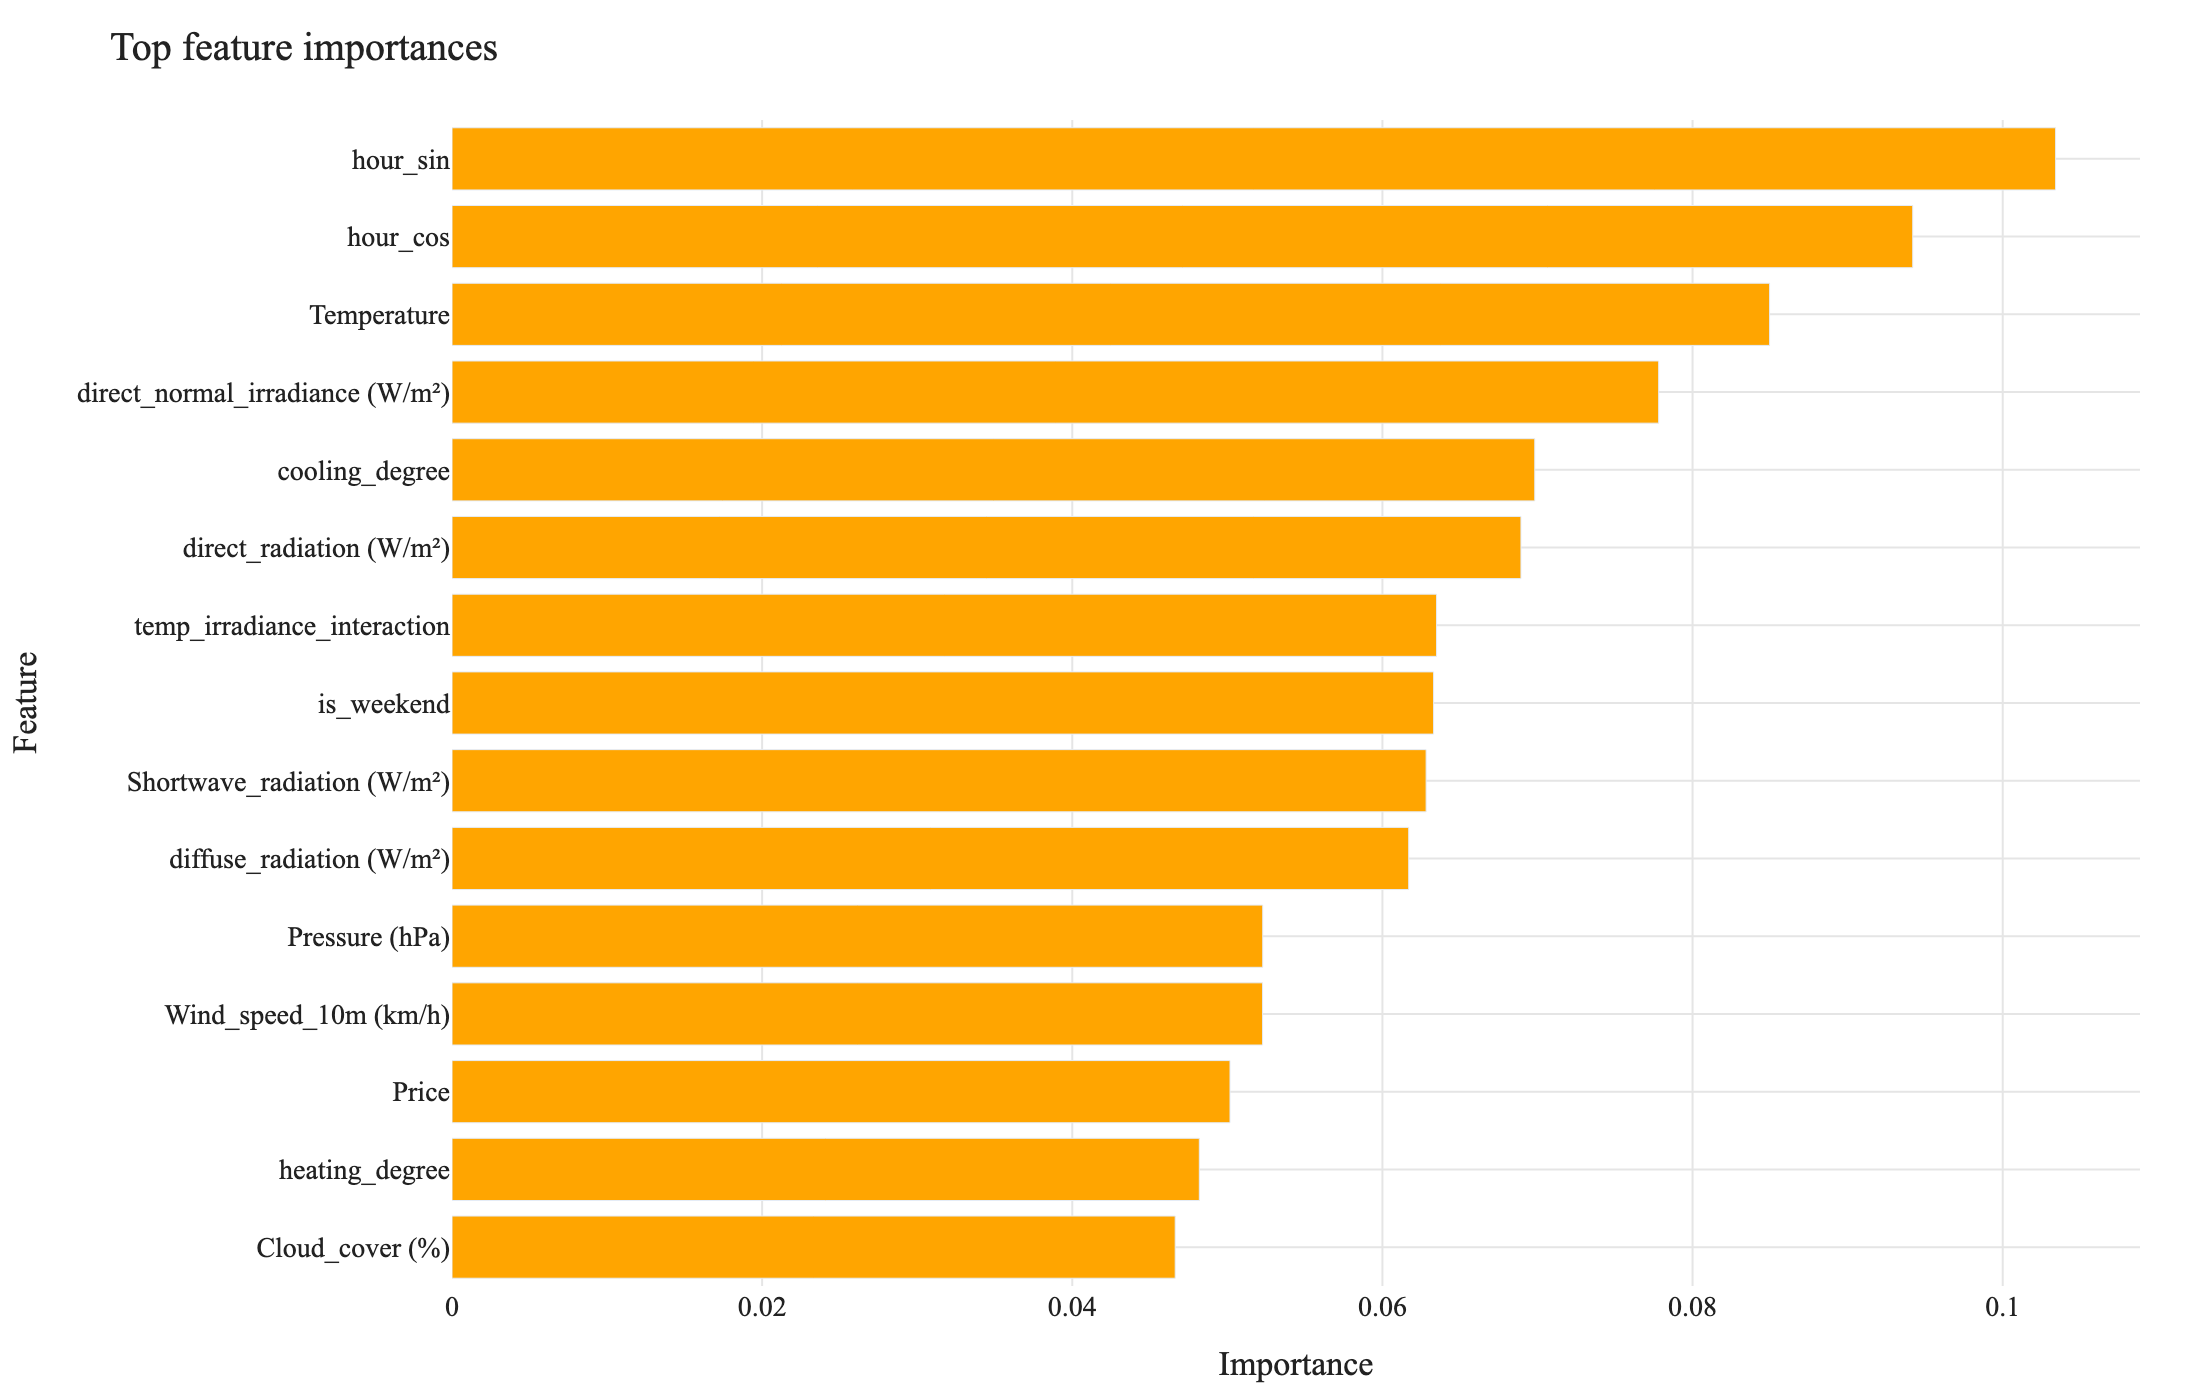
\includegraphics[width=\linewidth]{ml_feat_importance.png}
  \caption{Model-based feature importance.}
  \label{fig:ml_feat_importance}
\end{figure}

\begin{figure}[H]
  \centering
  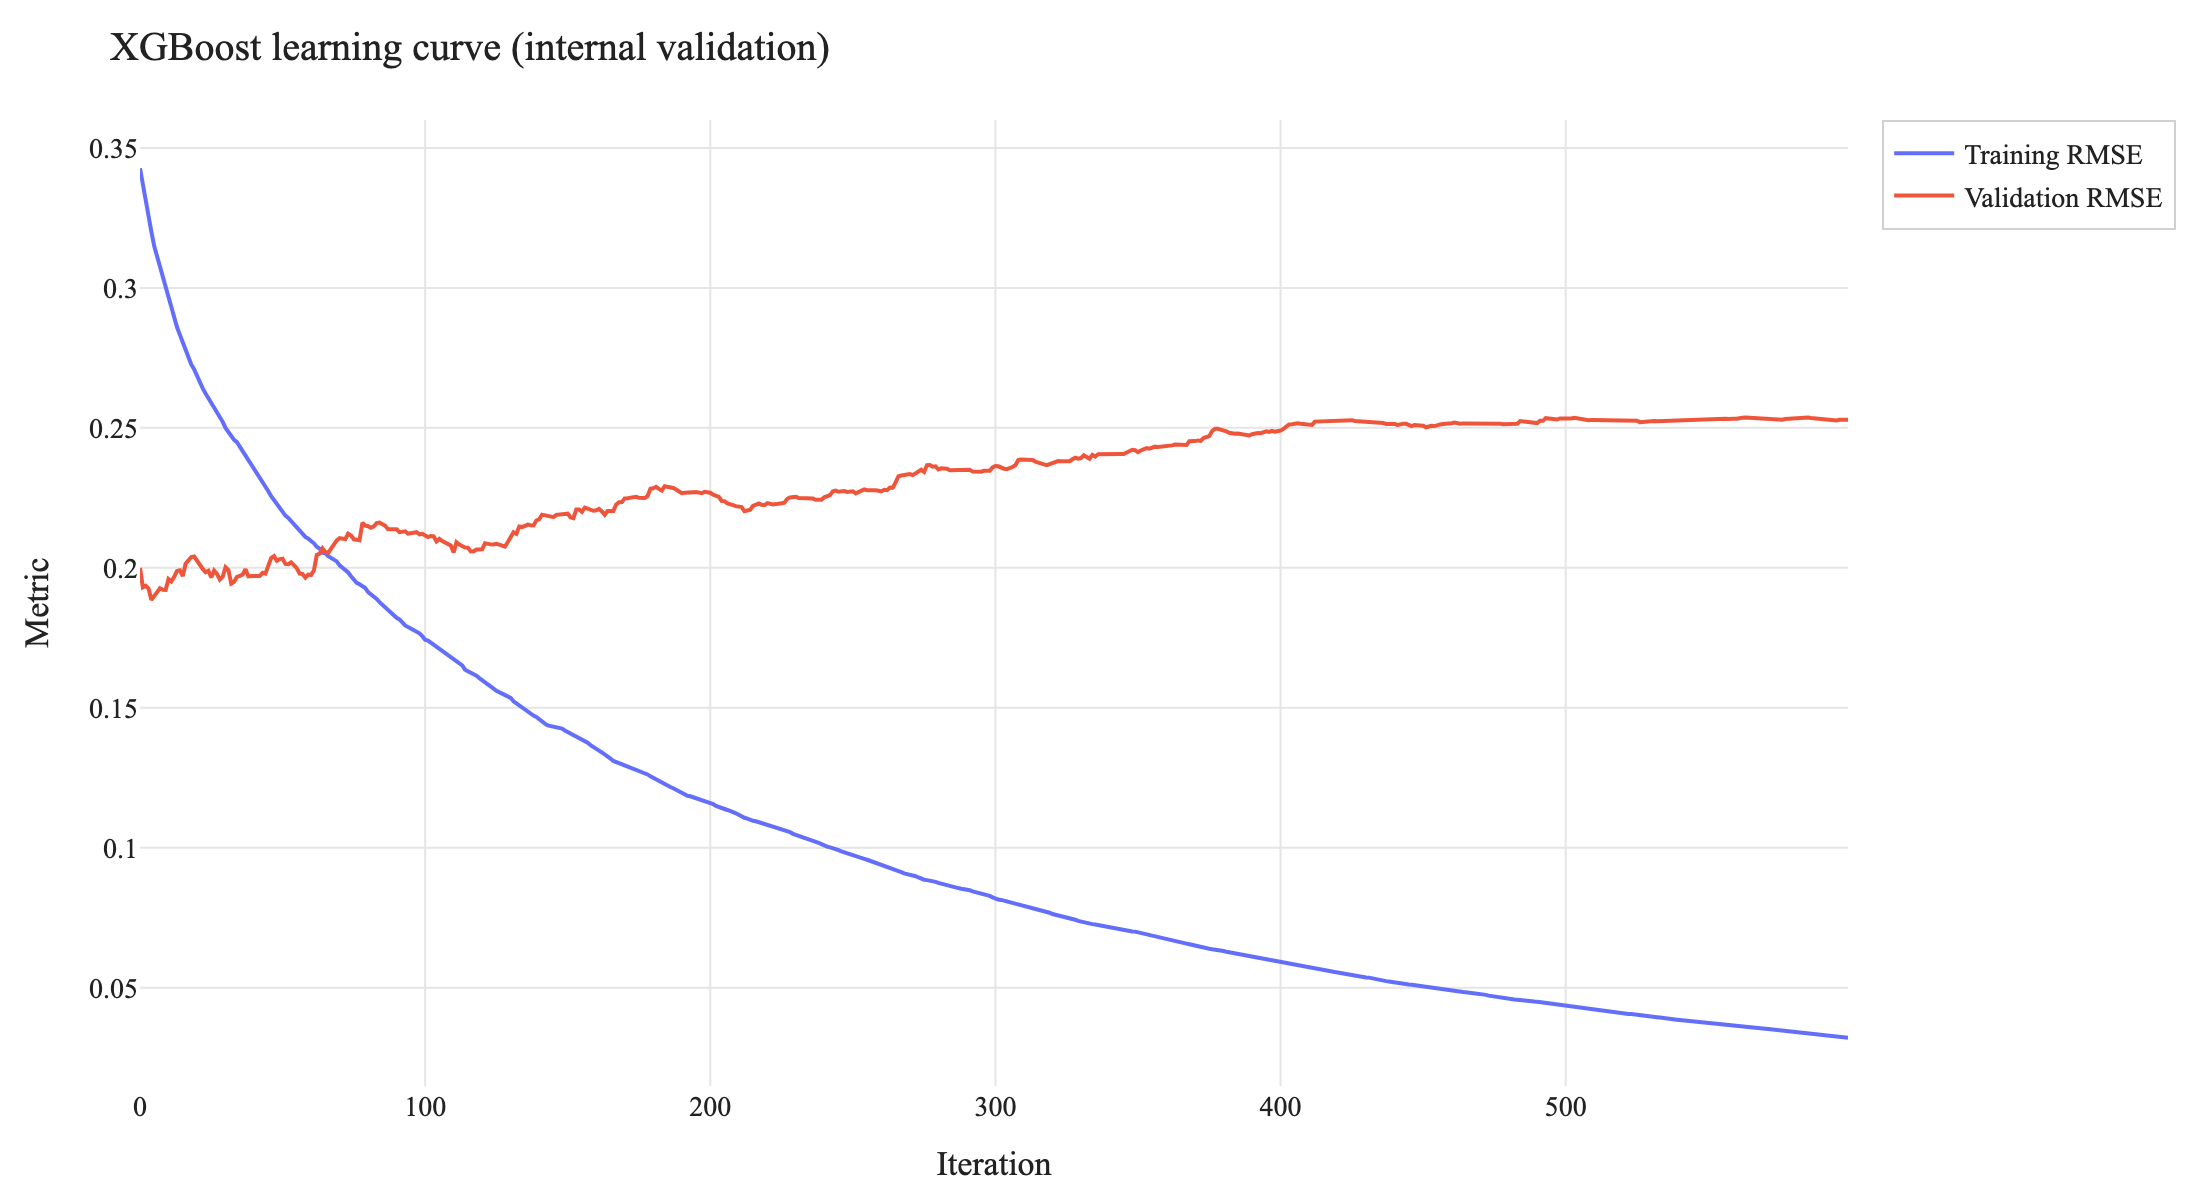
\includegraphics[width=\linewidth]{ml_learning_curve.png}
  \caption{Learning curve suggesting sufficient data volume.}
  \label{fig:ml_learning}
\end{figure}

\begin{figure}[H]
  \centering
  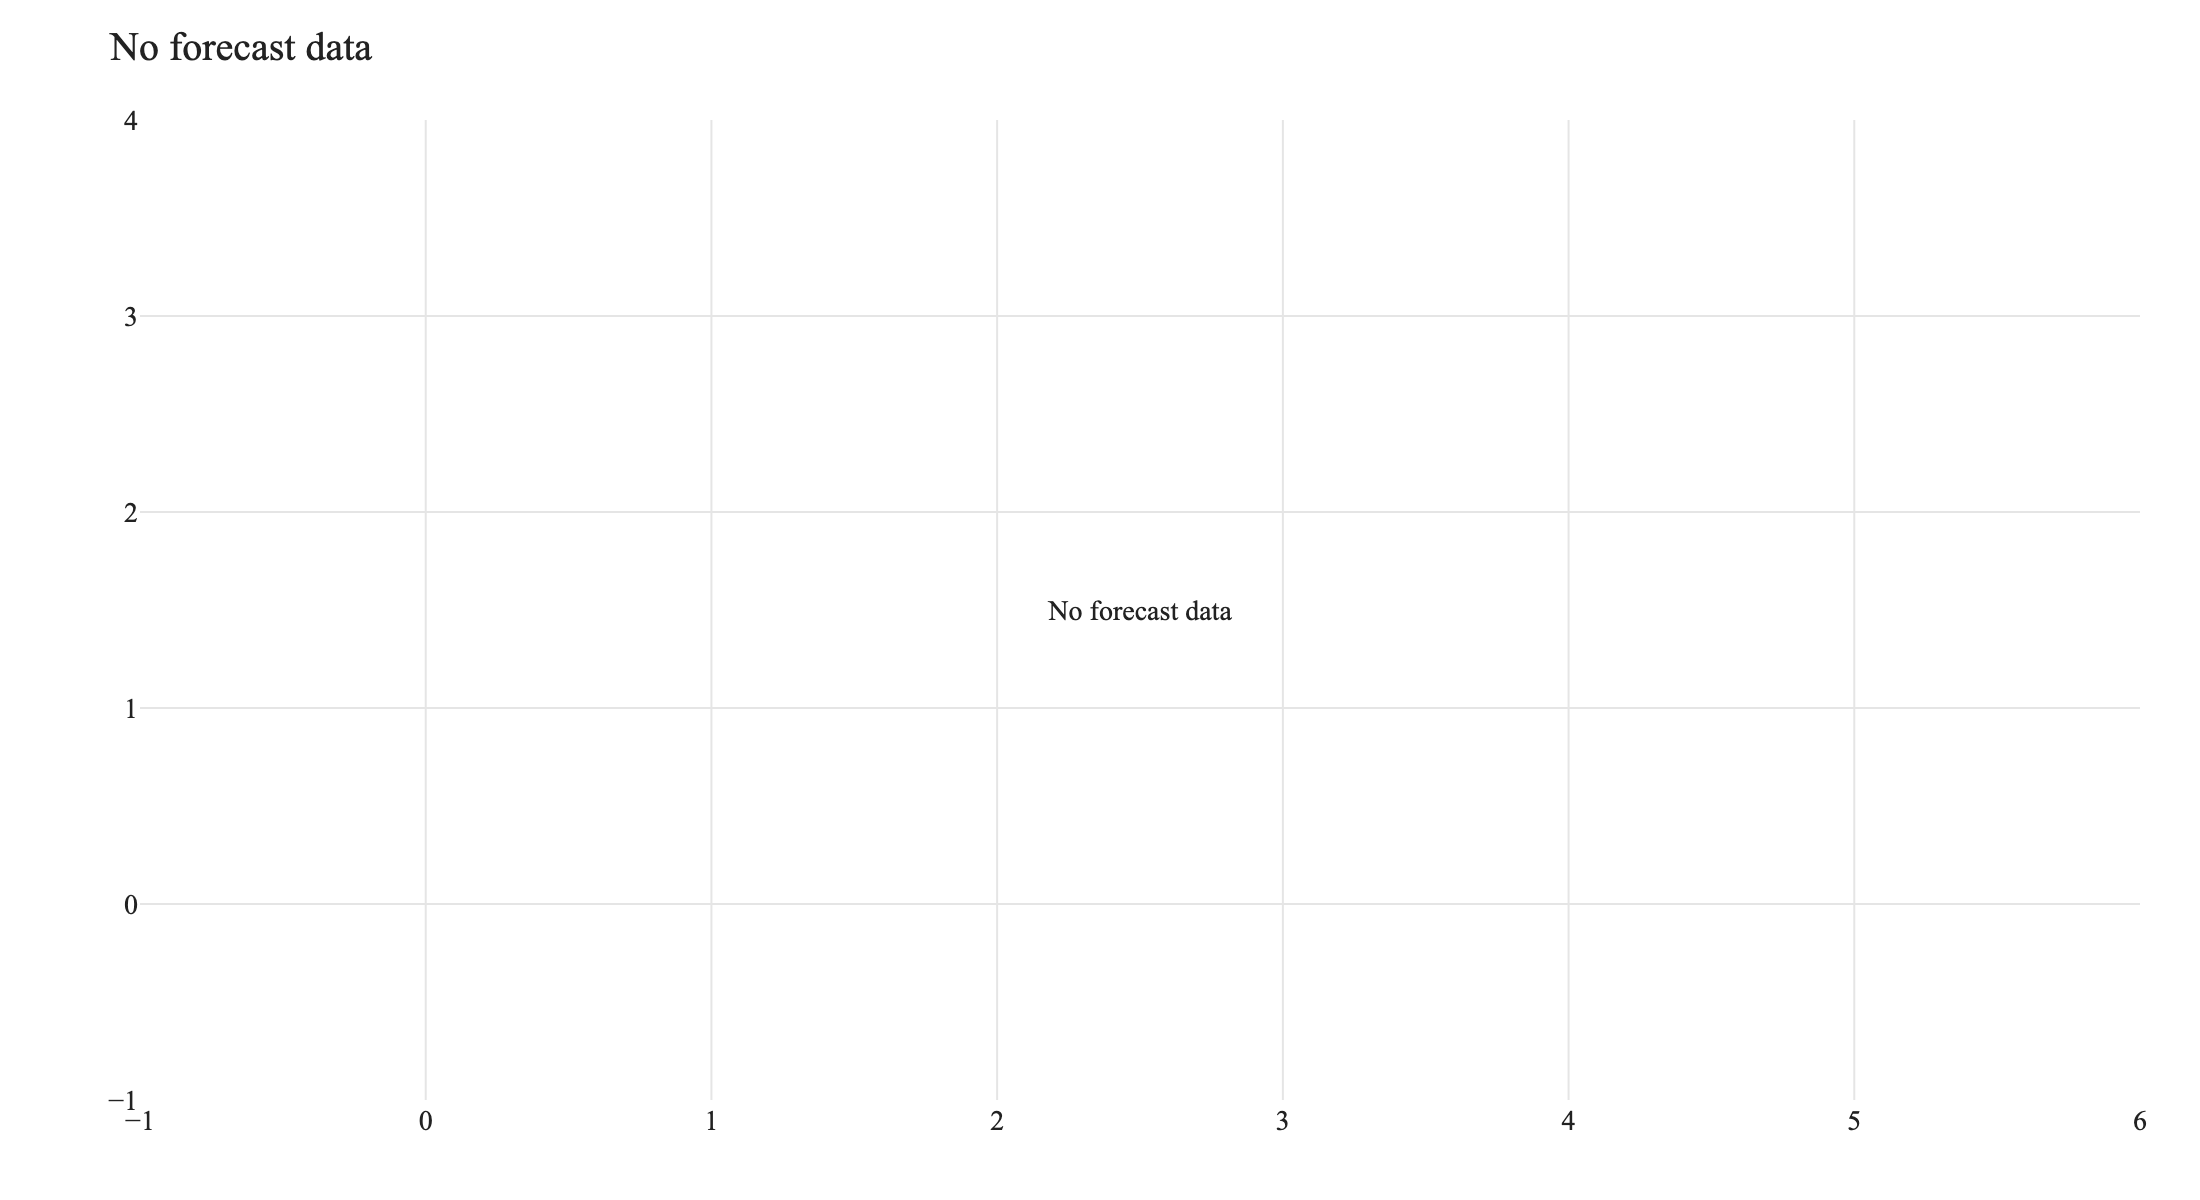
\includegraphics[width=\linewidth]{ml_forecast_overlay.png}
  \caption{ML forecast overlay on hold-out period.}
  \label{fig:ml_overlay}
\end{figure}

\begin{figure}[H]
  \centering
  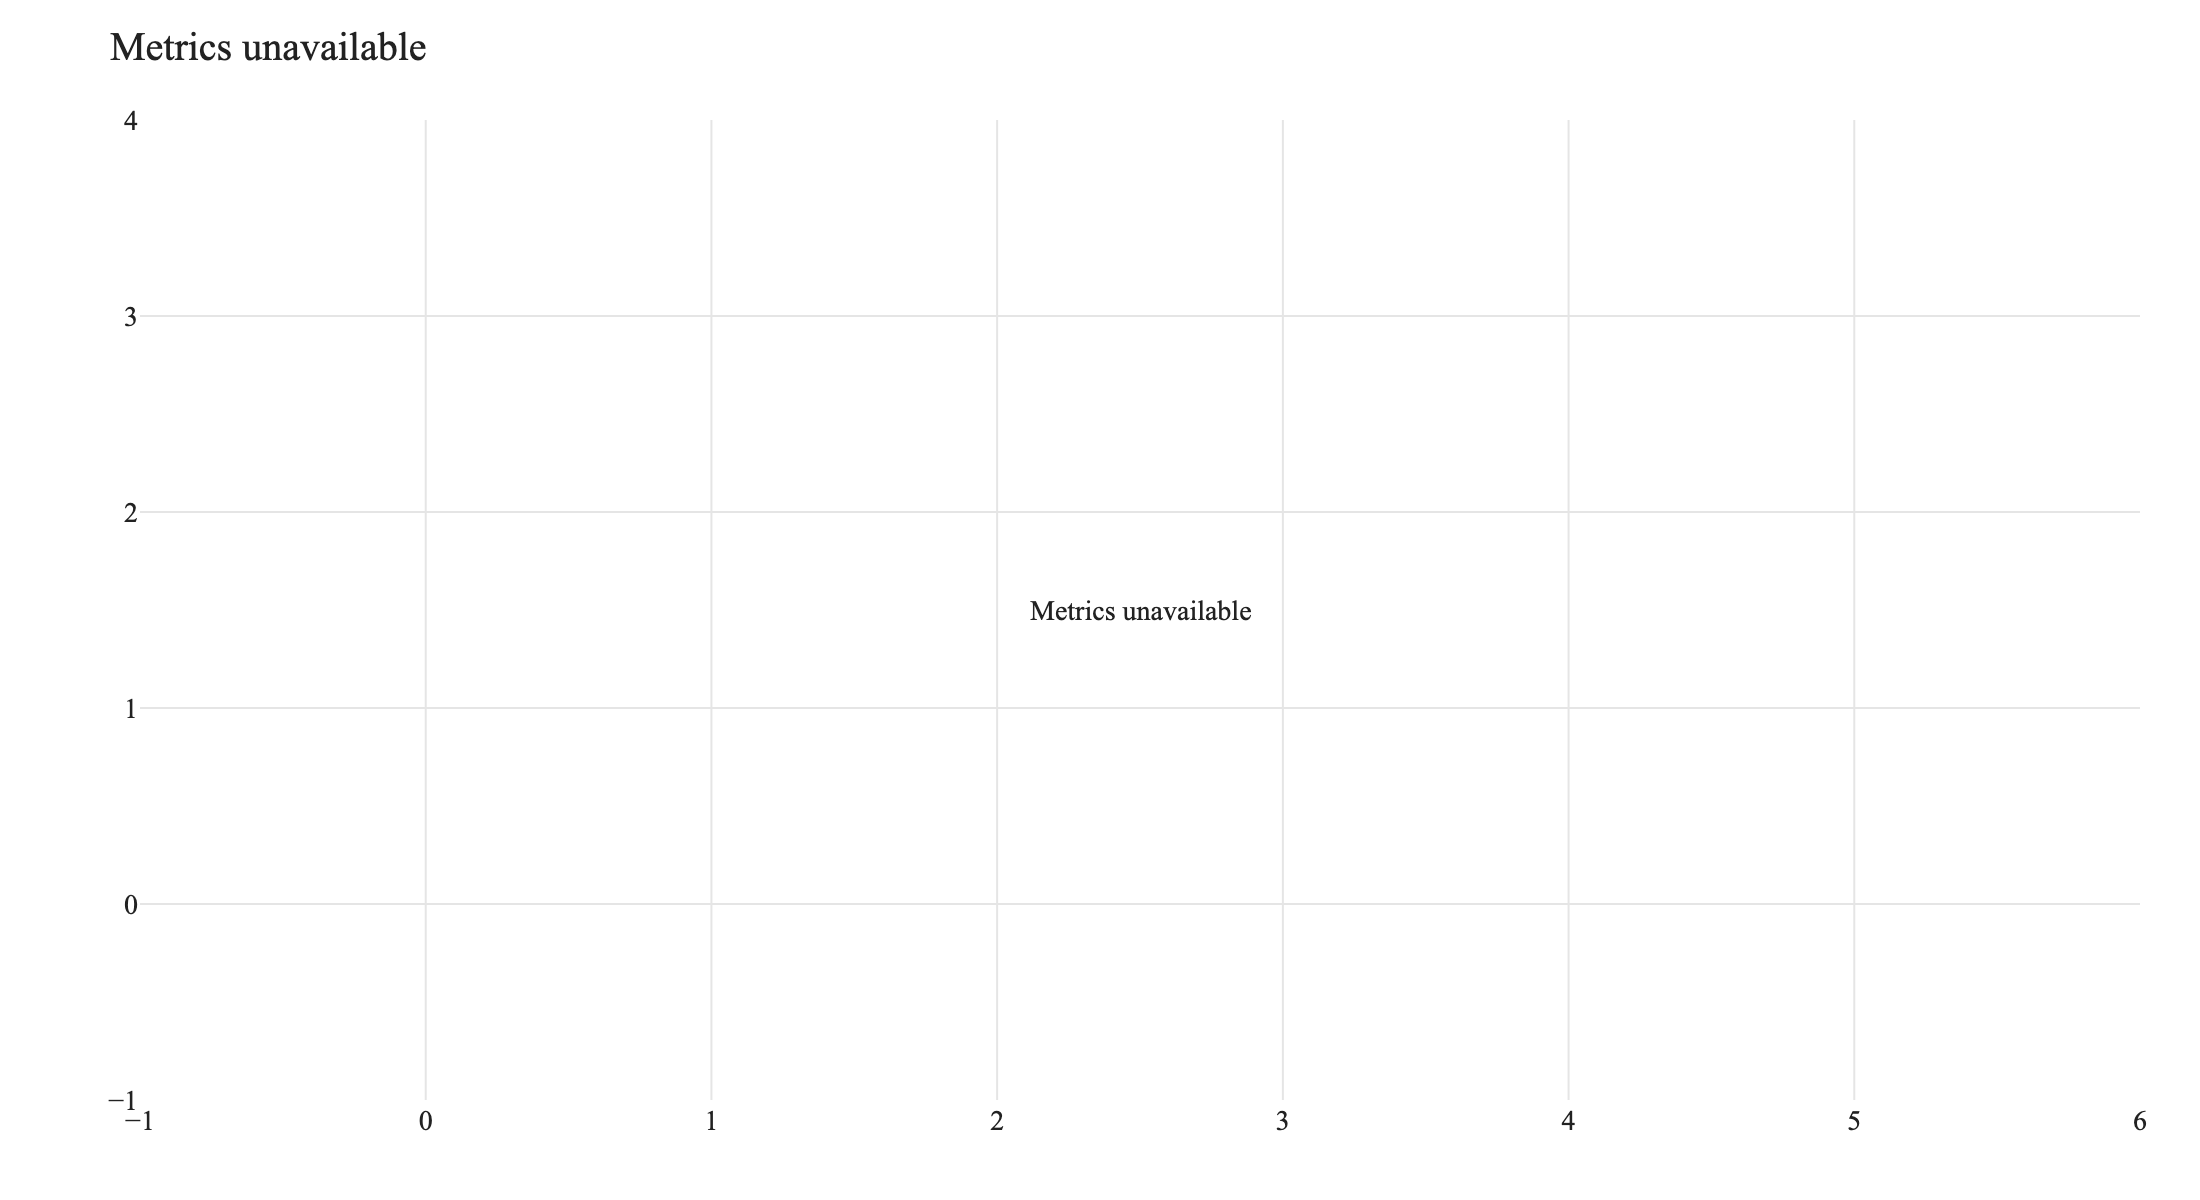
\includegraphics[width=\linewidth]{ml_metrics_comparison.png}
  \caption{Comparison of ML metrics against statistical baselines.}
  \label{fig:ml_metrics}
\end{figure}

%===========================
% 9. Forecasting Pipeline
%===========================
\section{Forecasting Pipeline}
A rolling 7-day pipeline standardizes input processing, feature assembly, model prediction, and metric logging. Baselines include persistence (lag-24) and seasonal averages.

\begin{figure}[H]
  \centering
  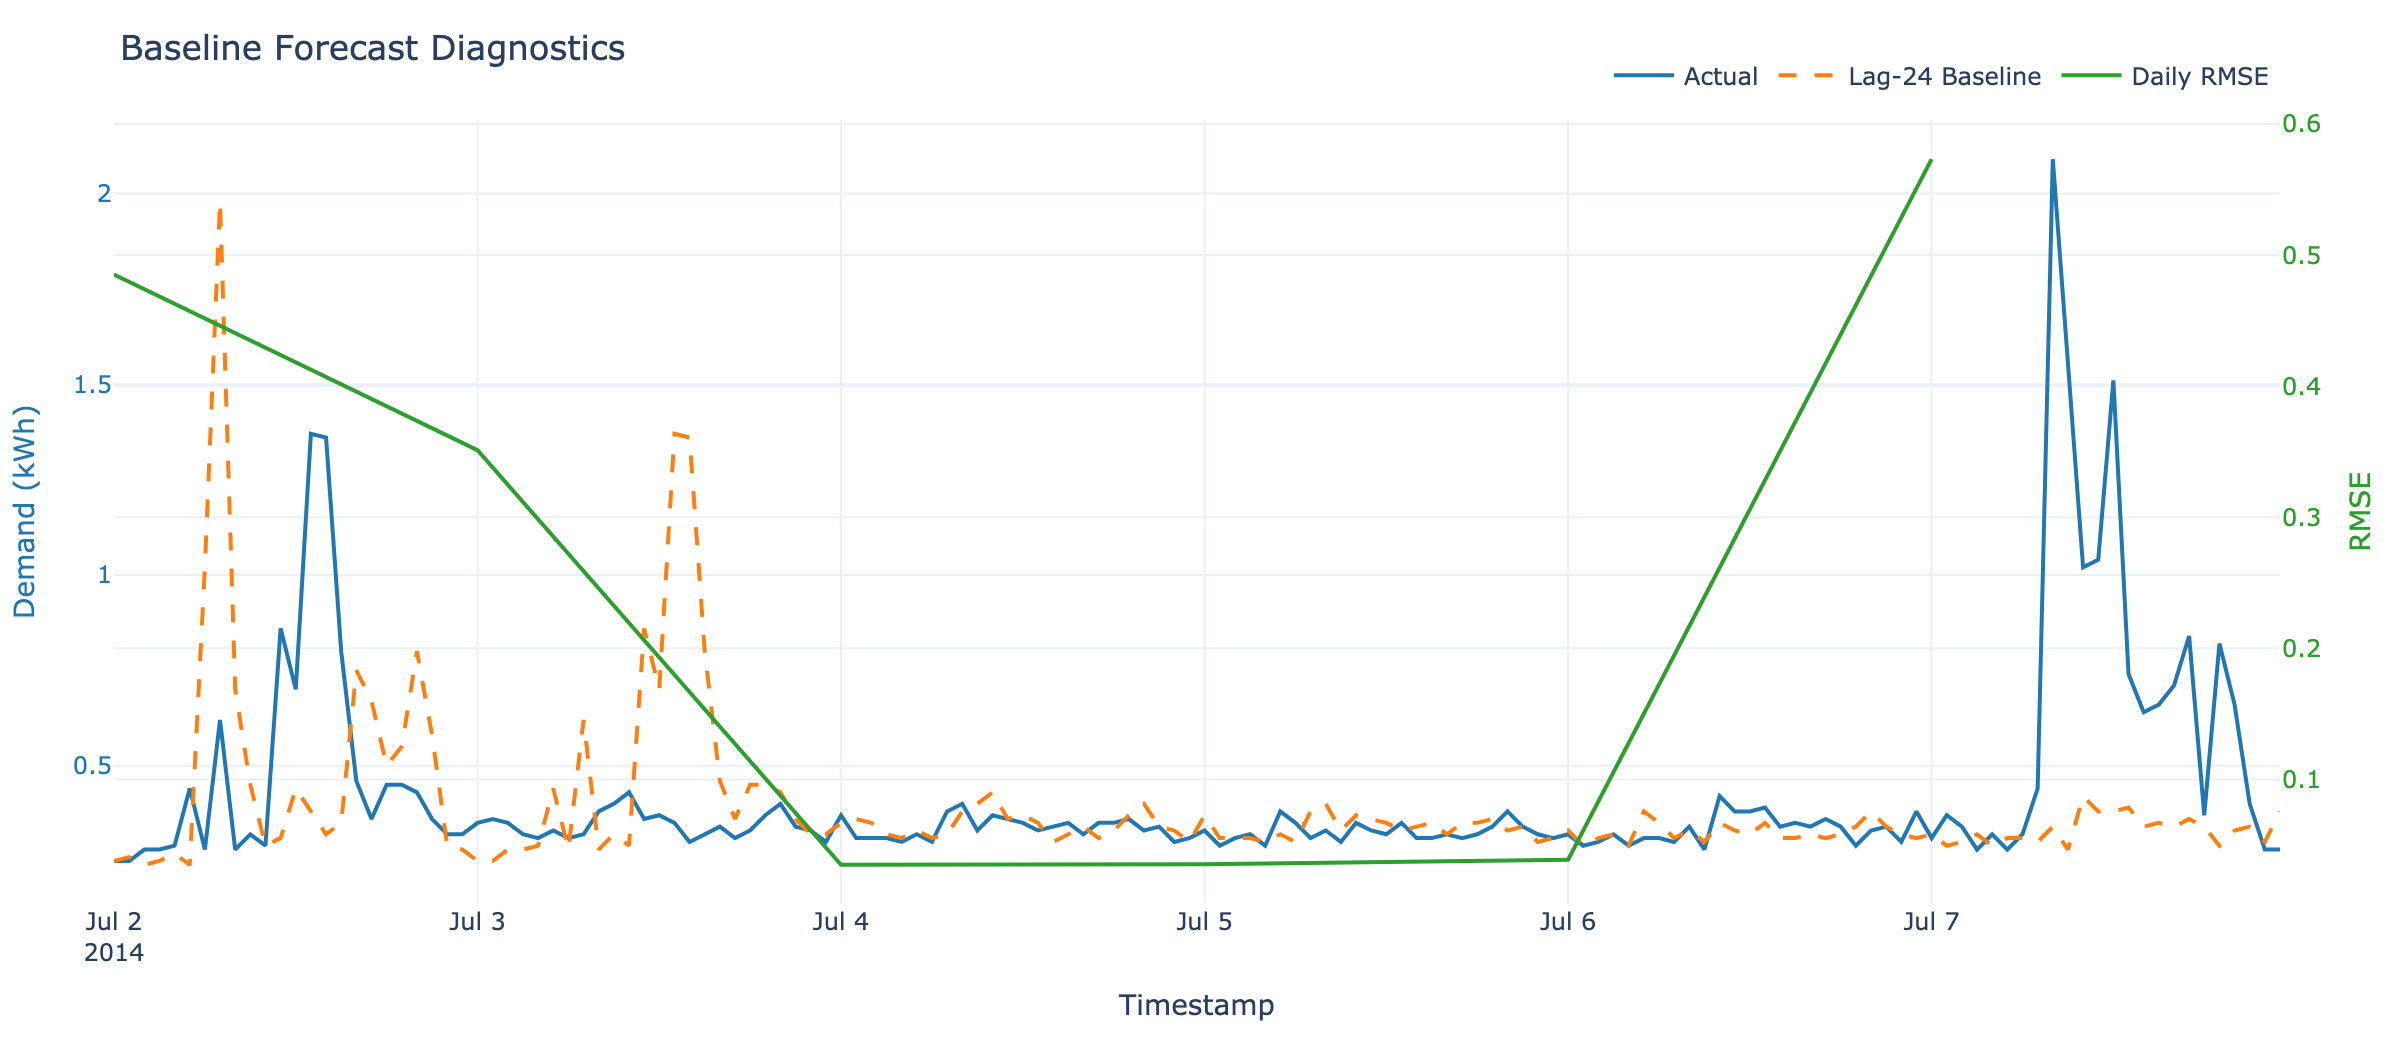
\includegraphics[width=\linewidth]{06_baseline_diagnostics.png}
  \caption{Baseline diagnostics (persistence), including daily RMSE.}
  \label{fig:baseline}
\end{figure}

%===========================
% 10. Exogenous Models
%===========================
\section{Models with Exogenous Inputs}
Exogenous features (temperature, calendar variables, PV) improved short-horizon forecasts. KPI summaries are provided in tables generated by the notebooks.

%===========================
% 11. Optimal Storage Control
%===========================
\section{Optimal Control of Energy Storage}
We formulate a cost-minimizing problem for a residential battery with SoC dynamics, power/energy limits, and tariff signals. The optimizer schedules charge/discharge to reduce imports and increase self-consumption.

%===========================
% 12. Discussion
%===========================
\section{Discussion and Critical Analysis}
Forecast-driven control curtails imports during peak prices, shifting demand to PV hours. ML with exogenous inputs typically outperforms ARIMA; statistical models remain valuable for interpretability. Limitations include single-household scope, potential concept drift, and tariff simplicity.

%===========================
% 13. Conclusion
%===========================
\section{Conclusion}
We demonstrate a complete HEMS analytics chain from raw data to operational optimization. Future work should incorporate uncertainty-aware forecasts, real-time adaptation, and richer tariff structures.

%===========================
% References
%===========================
\printbibliography

\end{document}
